% Options for packages loaded elsewhere
\PassOptionsToPackage{unicode}{hyperref}
\PassOptionsToPackage{hyphens}{url}
\PassOptionsToPackage{dvipsnames,svgnames,x11names}{xcolor}
%
\documentclass[
  11pt,
]{krantz}
\usepackage{amsmath,amssymb}
\usepackage{lmodern}
\usepackage{iftex}
\ifPDFTeX
  \usepackage[T1]{fontenc}
  \usepackage[utf8]{inputenc}
  \usepackage{textcomp} % provide euro and other symbols
\else % if luatex or xetex
  \usepackage{unicode-math}
  \defaultfontfeatures{Scale=MatchLowercase}
  \defaultfontfeatures[\rmfamily]{Ligatures=TeX,Scale=1}
  \setmonofont[Scale=0.775]{MesloLGS NF}
\fi
% Use upquote if available, for straight quotes in verbatim environments
\IfFileExists{upquote.sty}{\usepackage{upquote}}{}
\IfFileExists{microtype.sty}{% use microtype if available
  \usepackage[]{microtype}
  \UseMicrotypeSet[protrusion]{basicmath} % disable protrusion for tt fonts
}{}
\makeatletter
\@ifundefined{KOMAClassName}{% if non-KOMA class
  \IfFileExists{parskip.sty}{%
    \usepackage{parskip}
  }{% else
    \setlength{\parindent}{0pt}
    \setlength{\parskip}{6pt plus 2pt minus 1pt}}
}{% if KOMA class
  \KOMAoptions{parskip=half}}
\makeatother
\usepackage{xcolor}
\IfFileExists{xurl.sty}{\usepackage{xurl}}{} % add URL line breaks if available
\IfFileExists{bookmark.sty}{\usepackage{bookmark}}{\usepackage{hyperref}}
\hypersetup{
  pdftitle={Appunti di Costruzione e validazione di strumenti di misura dell'efficacia dell'intervento psicologico in neuropsicologia -- B020881 (B213)},
  pdfauthor={Corrado Caudek},
  colorlinks=true,
  linkcolor={Maroon},
  filecolor={Maroon},
  citecolor={Blue},
  urlcolor={Blue},
  pdfcreator={LaTeX via pandoc}}
\urlstyle{same} % disable monospaced font for URLs
\usepackage{color}
\usepackage{fancyvrb}
\newcommand{\VerbBar}{|}
\newcommand{\VERB}{\Verb[commandchars=\\\{\}]}
\DefineVerbatimEnvironment{Highlighting}{Verbatim}{commandchars=\\\{\}}
% Add ',fontsize=\small' for more characters per line
\usepackage{framed}
\definecolor{shadecolor}{RGB}{248,248,248}
\newenvironment{Shaded}{\begin{snugshade}}{\end{snugshade}}
\newcommand{\AlertTok}[1]{\textcolor[rgb]{0.33,0.33,0.33}{#1}}
\newcommand{\AnnotationTok}[1]{\textcolor[rgb]{0.37,0.37,0.37}{\textbf{\textit{#1}}}}
\newcommand{\AttributeTok}[1]{\textcolor[rgb]{0.61,0.61,0.61}{#1}}
\newcommand{\BaseNTok}[1]{\textcolor[rgb]{0.06,0.06,0.06}{#1}}
\newcommand{\BuiltInTok}[1]{#1}
\newcommand{\CharTok}[1]{\textcolor[rgb]{0.5,0.5,0.5}{#1}}
\newcommand{\CommentTok}[1]{\textcolor[rgb]{0.37,0.37,0.37}{\textit{#1}}}
\newcommand{\CommentVarTok}[1]{\textcolor[rgb]{0.37,0.37,0.37}{\textbf{\textit{#1}}}}
\newcommand{\ConstantTok}[1]{\textcolor[rgb]{0,0,0}{#1}}
\newcommand{\ControlFlowTok}[1]{\textcolor[rgb]{0.27,0.27,0.27}{\textbf{#1}}}
\newcommand{\DataTypeTok}[1]{\textcolor[rgb]{0.27,0.27,0.27}{#1}}
\newcommand{\DecValTok}[1]{\textcolor[rgb]{0.06,0.06,0.06}{#1}}
\newcommand{\DocumentationTok}[1]{\textcolor[rgb]{0.37,0.37,0.37}{\textbf{\textit{#1}}}}
\newcommand{\ErrorTok}[1]{\textcolor[rgb]{0.14,0.14,0.14}{\textbf{#1}}}
\newcommand{\ExtensionTok}[1]{#1}
\newcommand{\FloatTok}[1]{\textcolor[rgb]{0.06,0.06,0.06}{#1}}
\newcommand{\FunctionTok}[1]{\textcolor[rgb]{0,0,0}{#1}}
\newcommand{\ImportTok}[1]{#1}
\newcommand{\InformationTok}[1]{\textcolor[rgb]{0.37,0.37,0.37}{\textbf{\textit{#1}}}}
\newcommand{\KeywordTok}[1]{\textcolor[rgb]{0.27,0.27,0.27}{\textbf{#1}}}
\newcommand{\NormalTok}[1]{#1}
\newcommand{\OperatorTok}[1]{\textcolor[rgb]{0.43,0.43,0.43}{\textbf{#1}}}
\newcommand{\OtherTok}[1]{\textcolor[rgb]{0.37,0.37,0.37}{#1}}
\newcommand{\PreprocessorTok}[1]{\textcolor[rgb]{0.37,0.37,0.37}{\textit{#1}}}
\newcommand{\RegionMarkerTok}[1]{#1}
\newcommand{\SpecialCharTok}[1]{\textcolor[rgb]{0,0,0}{#1}}
\newcommand{\SpecialStringTok}[1]{\textcolor[rgb]{0.5,0.5,0.5}{#1}}
\newcommand{\StringTok}[1]{\textcolor[rgb]{0.5,0.5,0.5}{#1}}
\newcommand{\VariableTok}[1]{\textcolor[rgb]{0,0,0}{#1}}
\newcommand{\VerbatimStringTok}[1]{\textcolor[rgb]{0.5,0.5,0.5}{#1}}
\newcommand{\WarningTok}[1]{\textcolor[rgb]{0.37,0.37,0.37}{\textbf{\textit{#1}}}}
\usepackage{longtable,booktabs,array}
\usepackage{calc} % for calculating minipage widths
% Correct order of tables after \paragraph or \subparagraph
\usepackage{etoolbox}
\makeatletter
\patchcmd\longtable{\par}{\if@noskipsec\mbox{}\fi\par}{}{}
\makeatother
% Allow footnotes in longtable head/foot
\IfFileExists{footnotehyper.sty}{\usepackage{footnotehyper}}{\usepackage{footnote}}
\makesavenoteenv{longtable}
\usepackage{graphicx}
\makeatletter
\def\maxwidth{\ifdim\Gin@nat@width>\linewidth\linewidth\else\Gin@nat@width\fi}
\def\maxheight{\ifdim\Gin@nat@height>\textheight\textheight\else\Gin@nat@height\fi}
\makeatother
% Scale images if necessary, so that they will not overflow the page
% margins by default, and it is still possible to overwrite the defaults
% using explicit options in \includegraphics[width, height, ...]{}
\setkeys{Gin}{width=\maxwidth,height=\maxheight,keepaspectratio}
% Set default figure placement to htbp
\makeatletter
\def\fps@figure{htbp}
\makeatother
\setlength{\emergencystretch}{3em} % prevent overfull lines
\providecommand{\tightlist}{%
  \setlength{\itemsep}{0pt}\setlength{\parskip}{0pt}}
\setcounter{secnumdepth}{5}
\usepackage{amsmath}
\usepackage{amssymb}
\usepackage{amsfonts}

\defaultfontfeatures{Scale=MatchLowercase}

\usepackage{booktabs}
\usepackage{longtable}
\usepackage[bf,singlelinecheck=off]{caption}

\usepackage{framed,color}
\definecolor{shadecolor}{RGB}{248,248,248}

\renewcommand{\textfraction}{0.05}
\renewcommand{\topfraction}{0.8}
\renewcommand{\bottomfraction}{0.8}
\renewcommand{\floatpagefraction}{0.75}

\renewenvironment{quote}{\begin{VF}}{\end{VF}}
\let\oldhref\href
\renewcommand{\href}[2]{#2\footnote{\url{#1}}}

\ifxetex
  \usepackage{letltxmacro}
  \setlength{\XeTeXLinkMargin}{1pt}
  \LetLtxMacro\SavedIncludeGraphics\includegraphics
  \def\includegraphics#1#{% #1 catches optional stuff (star/opt. arg.)
    \IncludeGraphicsAux{#1}%
  }%
  \newcommand*{\IncludeGraphicsAux}[2]{%
    \XeTeXLinkBox{%
      \SavedIncludeGraphics#1{#2}%
    }%
  }%
\fi

\makeatletter
\newenvironment{kframe}{%
\medskip{}
\setlength{\fboxsep}{.8em}
 \def\at@end@of@kframe{}%
 \ifinner\ifhmode%
  \def\at@end@of@kframe{\end{minipage}}%
  \begin{minipage}{\columnwidth}%
 \fi\fi%
 \def\FrameCommand##1{\hskip\@totalleftmargin \hskip-\fboxsep
 \colorbox{shadecolor}{##1}\hskip-\fboxsep
     % There is no \\@totalrightmargin, so:
     \hskip-\linewidth \hskip-\@totalleftmargin \hskip\columnwidth}%
 \MakeFramed {\advance\hsize-\width
   \@totalleftmargin\z@ \linewidth\hsize
   \@setminipage}}%
 {\par\unskip\endMakeFramed%
 \at@end@of@kframe}
\makeatother

\renewenvironment{Shaded}{\begin{kframe}}{\end{kframe}}

\usepackage{makeidx}
\makeindex

\urlstyle{tt}

\usepackage{amsthm}
\makeatletter
\def\thm@space@setup{%
  \thm@preskip=8pt plus 2pt minus 4pt
  \thm@postskip=\thm@preskip
}
\makeatother

\DeclareMathOperator{\V}{\mathbb{V}} % Define variance operator
\DeclareMathOperator{\Var}{\mathbb{V}} % Define variance operator
\DeclareMathOperator{\SD}{SD} % Define sd operator
\DeclareMathOperator{\Cov}{Cov} % Define covariance operator
\DeclareMathOperator{\Corr}{Corr} % Define correlation operator
\DeclareMathOperator{\Me}{Me} % Define mediane operator
\DeclareMathOperator{\Mo}{Mo} % Define mode operator

\DeclareMathOperator{\Bin}{Binomial} % Define binomial operator
\DeclareMathOperator{\Bernoulli}{Bernoulli} % Define Bernoulli operator
\DeclareMathOperator{\Ber}{\mathscr{B}} % Define Bernoulli operator
\DeclareMathOperator{\Poi}{Poisson} % Define Poisson operator
\DeclareMathOperator{\Uniform}{Uniform} % Define Uniform operator
\DeclareMathOperator{\Cauchy}{Cauchy} % Define Cauchy operator
\DeclareMathOperator{\B}{B} % beta function
% \mbox{B}(a, b) % beta function
% \mbox{Beta}(a, b) % beta distribution

\DeclareMathOperator{\elpd}{elpd} % Define elpd operator
\DeclareMathOperator{\lppd}{lppd} % Define lppd operator
\DeclareMathOperator{\LOO}{LOO} % Define LOO operator
\DeclareMathOperator{\argmin}{arg\,min} 
\DeclareMathOperator{\argmax}{arg\,max} 

\newcommand{\E}{\mathbb{E}} % Define expected value operator
\newcommand{\R}{\textsf{R}} % Define R programming language symbol
\newcommand{\Real}{\mathbb{R}} % Define real number operator
\newcommand{\Prob}{\mathscr{P}}
\newcommand{\indep}{\perp \!\!\! \perp}

\usepackage[
 labelfont=bf,
 font={small, it}
]{caption}
\usepackage{upquote} % print correct quotes in verbatim-environments
\usepackage{empheq}
\usepackage{xfrac}

\usepackage{polyglossia}
\setmainlanguage{italian}

\frontmatter
\ifLuaTeX
  \usepackage{selnolig}  % disable illegal ligatures
\fi
\usepackage[]{natbib}
\bibliographystyle{apalike}

\title{Appunti di Costruzione e validazione di strumenti di misura dell'efficacia dell'intervento psicologico in neuropsicologia -- B020881 (B213)}
\author{Corrado Caudek}
\date{2022-02-27}

\usepackage{amsthm}
\newtheorem{theorem}{Teorema}[chapter]
\newtheorem{lemma}{Lemma}[chapter]
\newtheorem{corollary}{Corollario}[chapter]
\newtheorem{proposition}{Proposizione}[chapter]
\newtheorem{conjecture}{Congettura}[chapter]
\theoremstyle{definition}
\newtheorem{definition}{Definizione}[chapter]
\theoremstyle{definition}
\newtheorem{example}{Esempio}[chapter]
\theoremstyle{definition}
\newtheorem{exercise}{Esercizio}[chapter]
\theoremstyle{definition}
\newtheorem{hypothesis}{Hypothesis}[chapter]
\theoremstyle{remark}
\newtheorem*{remark}{Osservazione}
\newtheorem*{solution}{Soluzione}
\begin{document}
\maketitle

\cleardoublepage\newpage\thispagestyle{empty}\null
% \cleardoublepage\newpage\thispagestyle{empty}\null
%\cleardoublepage\newpage
\thispagestyle{empty}
\begin{center}
\Large{Appunti di Costruzione e validazione di strumenti di misura dell'efficacia dell'intervento psicologico in neuropsicologia -- AA 2021/2022}

\vskip20pt

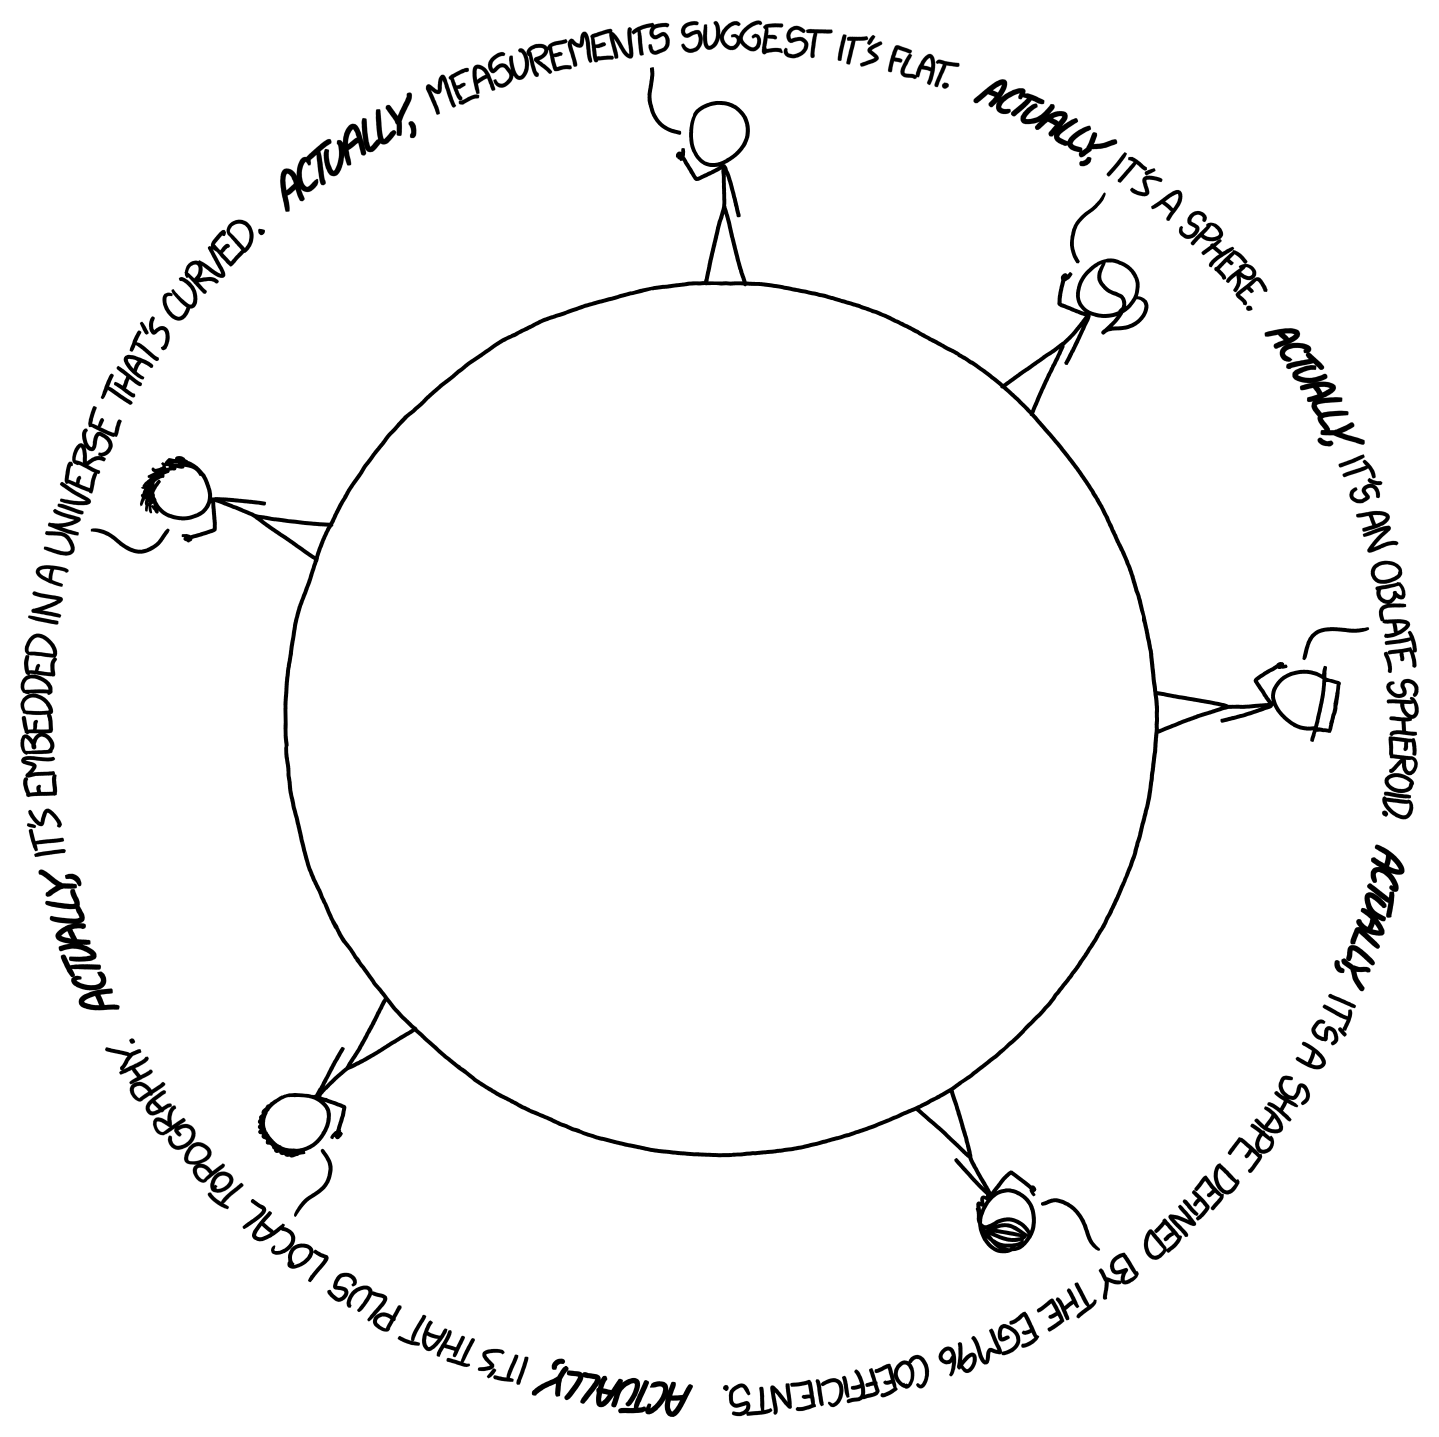
\includegraphics{images/actually_2x.png}
\end{center}

\setlength{\abovedisplayskip}{-5pt}
\setlength{\abovedisplayshortskip}{-5pt}

{
\hypersetup{linkcolor=}
\setcounter{tocdepth}{2}
\tableofcontents
}
\listoffigures
\listoftables
\hypertarget{prefazione}{%
\chapter*{Prefazione}\label{prefazione}}


La presente dispensa contiene il materiale delle lezioni dell'insegnamento di \emph{Costruzione e validazione di strumenti di misura dell'efficacia dell'intervento psicologico in neuropsicologia} B020881 (B213) rivolto agli studenti del secondo anno del Corso di Laurea Magistrale in Psicologia Clinica e della Salute e Neuropsicologia (curriculum: assessment e intervento psicologici in neuropsicologia - E21), A.A. 2021-2022. L'insegnamento si propone di fornire agli studenti un'introduzione all'assessment psicologico, ovvero un insieme di conoscenze/competenze che si pongono all'intersezione tra psicometria, statistica e informatica.

Nello specifico, l'insegnamento si focalizzerà sull'analisi fattoriale confermativa (\emph{confermatory factor analysis}, CFA) e sull'analisi fattoriale esplorativa, (\emph{explorative factor analysis}, EFA), cioè sugli strumenti che vengono usati durante il processo di sviluppo dei test psicometrici, ovvero che vengono usati per esaminare la struttura latente di una scala psicologica (ad esempio un questionario). In questo contesto, la CFA viene utilizzata per verificare il numero di dimensioni sottostanti gli indicatori (fattori) e l'intensità delle relazioni item-fattore (saturazioni fattoriali). La CFA consente anche di capire di come dovrebbe essere svolto lo scoring di un test. Quando la struttura latente è multifattoriale (cioè, a due o più fattori), il numero di fattori è indicativo del numero di sottoscale e di come esse dovrebbero essere codificate. La CFA è un importante strumento analitico anche per altri aspetti della valutazione psicometrica. Può essere utilizzata per stimare l'affidabilità di scala dei test psicometrici in modo da evitare i problemi della teoria classica dei test (ad es. alpha di Cronbach). Dati i recenti progressi nell'analisi dei dati categoriali, ora la CFA offre un quadro analitico comparabile a quello offerto dalla teoria di risposta agli item (IRT). In effetti, secondo \citet{brown2015confirmatory}, la CFA offre una maggiore flessibilità analitica rispetto al modello IRT tradizionale.

Un costrutto è un concetto teorico che può essere operazionalizzato nei termini di un fattore. In psicologia clinica, psichiatria e neuropsicologia, ad esempio, i disturbi mentali sono costrutti manifestati da vari insiemi di sintomi che sono riportati dal paziente o osservati da altri. La CFA è uno strumento analitico indispensabile per la validazione dei costrutti psicologici. I risultati della CFA possono fornire prove convincenti della validità convergente e discriminante dei costrutti teorici. La validità convergente è indicata dall'evidenza che diversi indicatori di costrutti teoricamente simili o sovrapposti sono fortemente correlati. La validità discriminante è indicata dai risultati che mostrano che gli indicatori di costrutti teoricamente distinti sono altamente incorrelati. Un punto di forza fondamentale degli approcci CFA per la costruzione e la validazione di uno strumento psicometrico è che le risultanti stime di validità convergente e discriminante sono corrette per l'errore di misurazione. Pertanto, la CFA fornisce un quadro analitico migliore rispetto ai metodi tradizionali che non tengono conto dell'errore di misurazione (ad esempio, gli approcci ordinari ai minimi quadrati come la correlazione/regressione multipla, i quali presuppongono che le variabili nell'analisi siano prive di errori di misurazione).

Spesso, parte della covariazione delle misure osservate è dovuta a fonti diverse dai fattori latenti di interesse. Questa covariazione aggiuntiva spesso riflette la varianza del metodo utilizzato per la misurazione. Gli effetti del metodo possono verificarsi anche all'interno di un'unica modalità di valutazione. Ad esempio, effetti del metodo sono solitamente presenti nei questionari che contengono una combinazione di elementi formulati positivamente e negativamente. Sfortunatamente, l'EFA non è in grado di stimare gli effetti del metodo. In effetti, l'uso di EFA quando esistono effetti del metodo può produrre risultati fuorvianti, ovvero suggerire la presenza di fattori aggiuntivi che corrispondono invece ad artefatti della misurazione. Nella CFA, invece, gli effetti del metodo possono essere specificati come parte della teoria dell'errore del modello di misurazione.

Un altro punto di forza della CFA è la sua capacità di affrontare il problema della generalizzabilità del modello di misurazione tra gruppi di individui o nel tempo. La valutazione dell'invarianza della misura è un aspetto importante dello sviluppo del test. Se un test è destinato a essere somministrato in una popolazione eterogenea, si dovrebbe stabilire che le sue proprietà di misurazione sono equivalenti in sottogruppi della popolazione (es. sesso, razza). Si dice che un test è distorto quando alcuni dei suoi elementi non misurano il costrutto sottostante in modo comparabile tra gruppi di rispondenti. Il test fornisce una stima distorta se, ad esempio, per un dato livello di vera intelligenza, gli uomini tendono a ottenere un punteggio di QI più alto rispetto alle donne. Il problema della generalizzabilità della validità del costrutto tra i gruppi può essere affrontato nella CFA esaminando gruppi multipli mediante modelli MIMIC (indicatori multipli, cause multiple). Inotre, è possibile chiedersi se il modello di misurazione sia equivalente tra i gruppi. Le soluzioni CFA a gruppi multipli vengono anche utilizzate per esaminare l'invarianza della misurazione longitudinale. Questo è un aspetto molto importante dell'analisi delle variabili latenti dei progetti di misure ripetute. In assenza di tale valutazione, non è possibile determinare se il cambiamento temporale in un costrutto sia dovuto a un vero cambiamento dei rispondenti o a cambiamenti nel modo di rispondere alla scala nel tempo. L'analisi a gruppi multipli può essere applicata a qualsiasi tipo di modello CFA. Ad esempio, queste procedure possono essere incorporate nell'analisi dei dati multitratto-multimetodo per esaminare la generalizzabilità della validità del costrutto tra gruppi.

In questo insegnamento la discussione delle teciche della CFA sarà preceduta da un'introduzione relativa alla EFA e la teoria classica dei test. La EFA, infatti, può essere concepita il metodo che viene utilizzato nei primi passi dello sviluppo di una scala psicometria, mentre la teoria classica dei test rappresenta la cornice teorica di partenza, di cui la CFA e i modelli di equazioni strutturali costituiscono uno sviluppo.

L'insegnamento pone una grande enfasi non solo sulla comprensione dei concetti teorici necessari per la costruzione e la validazione di uno strumento di misura in psicologia, ma anche sulla capacità di applicare tali concetti in situazioni concrete. Di conseguenza, la discussione dei concetti sarà sempre accompagnata da applicazioni pratiche. Tali applicazioni richiedono l'uso di un software. In questo insegnamento useremo \(\textsf{R}\) \citep{rmanual} quale linguaggio di programmazione probabilistica e, tra gli altri, il pacchetto \texttt{lavaan} che consente di svolgere le analisi statistiche della CFA e della EFA \citep{beaujean2014latent}. La teoria classica dei test verrà descritta con riferimento al classico testo di \citet{lord1968statistical}. Questa dispensa, inoltre, segue da vicino la trattazione della CFA fornita nei testi di \citet{mcdonald2013test} e di \citet{brown2015confirmatory}.

Trattando di argomenti avanzati, questo insegnamento presuppone la conoscenza di base dei concetti fondamentali della teoria delle probabilità; presuppone inoltre il possesso delle conoscenze di base necessarie per procedere all'utilizzo di \(\textsf{R}\). Informazioni su tali argomenti sono forniti nella dispensa di Psicometria (A.A. 2021-2022).

\begin{flushright}
Corrado Caudek\\
Marzo 2022 \end{flushright}

\mainmatter

\hypertarget{part-la-teoria-classica-dei-test}{%
\part{La teoria classica dei test}\label{part-la-teoria-classica-dei-test}}

\hypertarget{ch:teoria_classica}{%
\chapter{Fondamenti teorici}\label{ch:teoria_classica}}

\hypertarget{valutazione-psicometrica-come-ragionamento-inferenziale}{%
\section{Valutazione psicometrica come ragionamento inferenziale}\label{valutazione-psicometrica-come-ragionamento-inferenziale}}

In apparenza, i test psicometrici sono solo dei test. Somministriamo un test, otteniamo un punteggio ed è naturale pensare che sia tutto lì. Nonostante le apparenze, la valutazione psicologica e neuropsicologica non consiste soltanto nell'assegnare di punteggi: si tratta di ragionare su ciò che osserviamo di quello che le persone dicono, fanno o producono, in maniera tale da giungere a delle concezioni più ampie di tali persone a proposito di aspetti che non abbiamo -- e spesso non possiamo -- osservare. Più specificamente, possiamo considerare la valutazione psicologica e neuropsicologica come un esempio di ragionamento che fa uso di modelli probabilistici per giungere a delle spiegazioni, previsioni o conclusioni.

I dati osservati diventano un'evidenza quando sono ritenuti rilevanti per l'inferenza desiderata attraverso l'instaurazione di relazioni tra i dati e l'obiettivo dell'inferenza. Spesso utilizziamo dati provenienti da più fonti. Queste possono essere di tipo simile (ad esempio, item di test aventi lo stesso formato) o di tipo molto diverso (ad esempio, il curriculum di un richiedente oltre al colloquio, la storia medica della famiglia di un paziente, \(\dots\)). Le evidenze possono essere contraddittorie (ad esempio, uno studente riesce a svolgere un compito difficile ma fallisce in un uno facile) e quasi sempre non sono del tutto conclusive.

Queste caratteristiche hanno due implicazioni. In primo luogo, è difficile capire cosa le evidenze implicano. I processi inferenziali sono sempre complessi. In secondo luogo, a causa della natura non conclusiva delle evidenze disponibili, non siamo mai del tutto certi delle nostre inferenze. Per affrontare tale incertezza, la teoria psicometria ci fornisce gli strumenti che ci possono aiutare nel processo inferenziale, dai dati disponibili alle decisioni che prendiamo.

Un secolo fa, la relazione tra prestazioni osservate, da un lato, e l'abilità inosservabile del rispondente, dall'altro, iniziò a essere formalizzata nei termini dell'\emph{errore di misurazione}. \citet{gulliksen1961measurement} ha descritto ``il problema centrale della teoria dei test'' come ``la relazione tra l'abilità dell'individuo e il suo punteggio osservato sul test'' (p.~101). Tale caratterizzazione è valida ancora oggi, con una definizione opportunamente ampia di ``abilità'' e di ``punteggio sul test'' che sia in grado di comprendere le diverse forme di assessment psicologico e neuropsicologico. Comprendere e essere in grado di rappresentare la relazione tra le prestazioni osservate e la capacità soggiacente è dunque fondamentale per le forme di ragionamento che vengono impiegate nella valutazione psicologica e neuropsicologica.

Come risultato dell'errore di misurazione, i ragionamenti che compiamo nella valutazione psicologica e neuropsicologica costituiscono un esempio di ragionamento in condizioni di incertezza. A causa della natura imperfetta della misurazione e dell'incompletezza dell'informazione disponibile, le nostre inferenze sono incerte e possono essere sempre invalidate o riviste. Ragionare da ciò che è parziale (ciò che vediamo uno paziente dire, fare o produrre) a ciò che è generale (la ``vera'' abilità del paziente) è necessariamente incerto, e le nostre inferenze o conclusioni sono sempre prone ad errori.

Quali strumenti devono essere impiegati per affrontare la nostra incertezza sulla relazione che intercorre tra prestazioni osservate e abilità soggiacenti? Secondo Lewis, molti dei progressi nella teoria psicometrica sono resi possibili ``trattando lo studio della relazione tra le risposte agli item di un test e il tratto ipotizzato di un individuo come problema di inferenza statistica'' \citep{lewis1986test}. Una connessione diretta tra errore di misura e approccio probabilistico è stata anche proposta da Samejima: ``There may be an enormous number of factors eliciting a student's specific overt reactions to a stimulus, and, therefore, it is suitable, even necessary, to handle the situation in terms of the probabilistic relationship between the two'' \citep{samejima1983constant}.

Questo punto di vista è diventato quello dominante nella psicometria moderna e sottolinea l'utilità di utilizzare il linguaggio e gli strumenti della teoria della probabilità per comunicare il carattere parziale dei dati di cui dispone lo psicologo e l'incertezza delle inferenze che ne derivano.

I reattivi psicologici possono essere costruiti e la validati mediante vari approcci probabilistici: la Teoria Classica dei test (\emph{classical test theory}, in breve CTT) e la teoria di risposta all'item (\emph{item response theory}, in breve IRT) sono quelli più noti. Recentemente, il problema della valutazione psicologica è stato anche formulato in un'ottica bayesiana. In questo insegnamento esamineremo gli approcci della CTT e dell'IRT, ma non quello bayesiano.

\hypertarget{la-teoria-classica}{%
\section{La Teoria Classica}\label{la-teoria-classica}}

La CTT nasce alla fine dell'Ottocento (Alfred Binet e altri, 1894) allo scopo di studiare l'attendibilità e la validità dei risultati dei questionari utilizzati per valutare le caratteristiche psico-sociali, non direttamente osservabili, delle persone esaminate. L'impiego su vasta scala e lo sviluppo della CTT ha inizio negli anni Trenta, anche se il modello formale su cui tale teoria si basa viene proposta da Spearman all'inizio del Novecento \citep{ch1904general}. La tecnica dell'analisi fattoriale esplorativa (\emph{Exploratory Factor Analysis}, EFA), verrà poi affinata da \citet{thurstone1947multiple} alla fine della seconda guerra mondiale. Tra la fine degli anni '60 e gli inizi degli anni '70, \citet{joreskog1969general} sviluppa l'analisi fattoriale confermativa (\emph{Confirmatory Factor Analysis}, CFA). Negli anni '70, l'analisi fattoriale viene integrata con la path analysis nel lavoro di \citet{joreskog1978structural} che dà origine ai modelli di equazioni strutturali (\emph{Structural Equation Modeling}, SEM).

Iniziamo qui ad esaminare queste tecniche psicometriche prendendo in esame, per prima, la teoria classica dei test. Seguiremo la trattazione proposta da \citet{lord1968statistical}.

L'equazione fondamentale alla quale si riconduce la teoria classica dei test è quella che ipotizza una relazione lineare e additiva tra il punteggio osservato di un test (\(X\)), la misura della variabile latente (\(T\)) e la componente casuale dell'errore (\(E\)). Un punto cruciale nella CTT è l'entità della varianza dell'errore. Minore è la varianza dell'errore, più accuratamente il punteggio reale viene riflesso dai nostri punteggi osservati. In un mondo perfetto, tutti i valori di errore sarebbero uguali a 0. Cioè, ogni partecipante otterrebbe il punteggio esatto. Questo però non è possibile. Pertanto, abbiamo una certa varianza negli errori. La corrispondente deviazione standard di tali errori ha il un nome: si chiama \emph{errore standard di misurazione}, indicato da \(\sigma_E\). Uno dei principali obiettivi della CTT è quello di ottenere una stima di \(\sigma_E\).

\hypertarget{le-due-componenti-del-punteggio-osservato}{%
\section{Le due componenti del punteggio osservato}\label{le-due-componenti-del-punteggio-osservato}}

CTT si occupa delle relazioni tra \(X\), \(T\) ed \(E\). La CTT si basa su un modello relativamente semplice in cui il punteggio osservato, il punteggio vero (cioè l'abilità inosservabile del rispondente) e l'errore aleatoria di misurazione sono legati da una relazione lineare. Indicati con \(T_{\nu j}\) (\emph{true score}) l'abilità latente da misurare dell'individuo \(\nu\) nella prova \(j\), con \(X_{\nu j}\) la variabile osservata (\emph{observed score}) per l'individuo \(\nu\) nella prova \(j\) e con \(E_{\nu j}\) l'errore aleatorio di misurazione, il modello si rappresenta con

\[
X_{\nu j} = T_{\nu} + E_{\nu j}. 
\label{eq:observed-true-plus-error}
\]

Dunque, in base alla \eqref{eq:observed-true-plus-error} il punteggio osservato \(X_{\nu j}\) differisce da quello vero \(T_{\nu j}\) a causa di una componente di errore aleatoria \(E_{\nu j}\). Uno degli obiettivi centrali della CTT è quello di quantificare l'entità di tale errore. Vedremo come questa quantificazione verrà fornita nei termini dell'attendibilità del test. L'attendibilità (o affidabilità) rappresenta l'accuratezza con cui un test può misurare il punteggio vero (Coaley, 2014):

\begin{itemize}
\tightlist
\item
  Se l'attendibilità è grande, \(\sigma_E\) è piccolo: \(X\) ha un piccolo errore di misurazione e sarà vicino a \(T\).
\item
  Se l'attendibilità è piccola, \(\sigma_E\) è grande: \(X\) presenta un grande errore di misurazione e si discosterà molto da \(T\).
\end{itemize}

\hypertarget{il-punteggio-vero}{%
\subsection{Il punteggio vero}\label{il-punteggio-vero}}

La @ref(eq:observed-true\_plus-error) ci dice che il punteggio osservato è dato dalla somma di due componenti: una componente sistematica (il punteggio vero) e una componente aleatoria (l'errore di misurazione). Ma che cos'è il punteggio vero? La CTT considera un reattivo psicologico come una selezione aleatoria di item da un universo/popolazione di item attinenti al costrutto da misurare \citep{nunnally1994psychometric, kline2013handbook}. Se il reattivo psicologico viene concepito in questo modo, il punteggio vero diventa il punteggio che un rispondente otterrebbe se fosse misurato su tutto l'universo degli item proprio del costrutto in esame. L'errore di misurazione riflette dunque il grado in cui gli item che costituiscono il test non riescono a rappresentare l'intero universo degli item attinenti al costrutto.

In maniera equivalente, il punteggio vero può essere concepito come il punteggio non ``distorto'' da componenti estranee al costrutto, ovvero da effetti di apprendimento, fatica, memoria, motivazione, eccetera. Essendo concepita come del tutto aleatoria (ovvero, priva di qualunque natura sistematica), la componente aleatoria non introduce dei bias nella tendenza centrale della misurazione.

Il punteggio vero è concepito come un punteggio inosservabile che corrisponde al valore atteso di infinite realizzazioni del punteggio ottenuto:

\[
T = \E(X) \equiv \mu_X \equiv \mu_{T}.
\]

In altri termini, secondo la definizione di Lord e Novick (1968), e facendo riferimento a alla seconda definizione presentata sopra, il punteggio vero è concepito come la media dei punteggi che un soggetto otterrebbe se il test venisse somministrato ripetutamente nelle stesse condizioni, in assenza di effetti di apprendimento e/o fatica.

\hypertarget{somministrazioni-ripetute}{%
\subsection{Somministrazioni ripetute}\label{somministrazioni-ripetute}}

Nella formulazione del modello della CTT si possono distinguere due tipi di esperimenti aleatori: uno che considera l'unità di osservazione (l'individuo) come campionaria, l'altro che considera il punteggio, per un determinato individuo, come campionario. Un importante risultato è dato dall'unione dei due esperimenti, ovvero dalla dimostrazione che i risultati della CTT, la quale è stata sviluppata ipotizzando ipotetiche somministrazioni ripetute del test allo stesso individuo sotto le medesime condizioni, si generalizzano al caso di una singola somministrazione del test ad un campione di individui \citep{allen2001introduction}. In base a questo risultato, se consideriamo la somministrazione del test ad una popolazione di individui, allora diventa più facile dare un contenuto empirico alle quantità della CTT:

\begin{itemize}
\tightlist
\item
  \(\sigma^2_X\) è la varianza del punteggio osservato nella popolazione,
\item
  \(\sigma^2_T\) è la varianza dei punteggio vero nella popolazione,
\item
  \(\sigma^2_E\) è la varianza della componente d'errore nella popolazione.
\end{itemize}

\hypertarget{le-assunzioni-sul-punteggio-ottenuto}{%
\subsection{Le assunzioni sul punteggio ottenuto}\label{le-assunzioni-sul-punteggio-ottenuto}}

La CTT \emph{assume} che la media del punteggio osservato \(X\) sia uguale alla media del punteggio vero,

\[
\mu_X \equiv \mu_{T},
\label{eq:assunzione-media-x-media-t}
\]

in altri termini, assume che il punteggio osservato fornisca una stima statisticamente corretta dell'abilità latente (punteggio vero). In pratica, il punteggio osservato non sarà mai uguale all'abilità latente, ma corrisponde solo ad uno dei possibili punteggi che il soggetto può ottenere, subordinatamente alla sua abilità latente. L'errore della misura è la differenza tra il punteggio osservato e il punteggio vero: \(E \equiv X - T.\)

In base all'assunzione secondo cui il valore atteso dei punteggi è uguale alla media del valore vero, segue che

\[
\E(E) = \E(X - T) = \E(X) - \E(T) = \mu_{T} - \mu_{T} = 0,
\]

ovvero, il valore atteso degli errori è uguale a zero.

\hypertarget{lerrore-standard-della-misurazione-sigma_e}{%
\section{\texorpdfstring{L'errore standard della misurazione \(\sigma_E\)}{L'errore standard della misurazione \textbackslash sigma\_E}}\label{lerrore-standard-della-misurazione-sigma_e}}

La radice quadrata di \(\sigma^2_E\), ovvero la deviazione standard degli errori, è la quantità fondamentale della CTT ed è chiamata \emph{errore standard della misurazione}. La stima dell'errore standard della misurazione costituisce uno degli obiettivi più importanti della CTT. Ricordiamo che la deviazione standard è simile (non identica) alla media del valore assoluto degli scarti dei valori di una distribuzione dalla media. Possiamo dunque utilizzare questa proprietà per descrivere il modo in cui la CTT interpreta \(\sigma_E\).

L'\emph{errore standard della misurazione} \(\sigma_E\) ci dice qual è, approssimativamente, la variazione attesa del punteggio osservato, se il test venisse somministrato un'altra volta al rispondente nelle stesse condizioni.

\hypertarget{assiomi-della-teoria-classica}{%
\section{Assiomi della Teoria Classica}\label{assiomi-della-teoria-classica}}

La CTT \emph{assume} che gli errori siano delle variabili aleatorie incorrelate tra loro

\[
\rho(E_i, E_k \mid T) = 0, \qquad\text{con}\; i \neq k,
\]

e incorrelate con il punteggio vero,

\[
\rho(E, T) = 0,
\]

le quali seguono una distribuzione gaussiana con media zero e deviazione standard pari a \(\sigma_E\):

\[
E \sim \mathcal{N}(0, \sigma_E).
\]

La quantità \(\sigma_E\) è detta errore standard della misurazione.

Sulla base di tali assunzioni la CTT deriva la formula dell'attendibilità di un test. Si noti che le assunzioni della CTT hanno una corrispondenza puntuale con le assunzioni su cui si basa il modello di regressione lineare.

\hypertarget{lattendibilituxe0-del-test}{%
\section{L'attendibilità del test}\label{lattendibilituxe0-del-test}}

Il concetto di attendibilità è strettamente legato alla riproducibilità della misurazione: si riferisce al grado di stabilità, di coerenza interna e di precisione di una procedura di misurazione. Affinché una misurazione psicologica sia utile, deve produrre lo stesso risultato se viene applicata ripetutamente un determinato rispondente. Altri termini che vengono usati sono: affidabilità, costanza e credibilità.

Vedremo nel seguito come il coefficiente di attendibilità fornisce una stima della quota della varianza del punteggio osservato che può essere attribuita all'abilità latente (``punteggio vero'', cioè privo di errore di misurazione). In generale, un coefficiente di attendibilità maggiore di 0.80 viene ritenuto soddisfacente perché indica che l'80\% o più della varianza dei punteggi ottenuti è causata da ciò che il test intende misurare, anziché dall'errore di misurazione.

Per definire l'attendibilità, la CTT si serve di due quantità:

\begin{itemize}
\tightlist
\item
  la varianza del punteggio osservato,
\item
  la correlazione tra punteggio osservato e punteggio vero.
\end{itemize}

Vediamo come queste quantità possano essere ottenute sulla base delle assunzioni del modello statistico che sta alla base della CTT.

\hypertarget{la-varianza-del-punteggio-osservato}{%
\subsection{La varianza del punteggio osservato}\label{la-varianza-del-punteggio-osservato}}

La varianza del punteggio osservato \(X\) è uguale alla somma della varianza del punteggio vero e della varianza dell'errore di misurazione.

\begin{proof}
La varianza del punteggio osservato è uguale a

\[
\sigma^2_X =  \V(T+E) =  \sigma_T^2 + \sigma_E^2 + 2 \sigma_{TE}.
\label{eq:3-2-4}
\]

Dato che \(\sigma_{TE}=\rho_{TE}\sigma_T \sigma_E=0\), in quanto \(\rho_{TE}=0\), ne segue che

\[
\sigma^2_X =   \sigma_T^2 + \sigma_E^2.
\label{eq:var-sum}
\]
\end{proof}

\hypertarget{la-covarianza-tra-punteggio-osservato-e-punteggio-vero}{%
\subsection{La covarianza tra punteggio osservato e punteggio vero}\label{la-covarianza-tra-punteggio-osservato-e-punteggio-vero}}

La covarianza tra punteggio osservato \(X\) e punteggio vero \(T\) è uguale alla varianza del punteggio vero.

\begin{proof}
\begin{equation}
\begin{aligned}
\sigma_{X T} &= \E(XT) - \E(X)\E(T)\notag\\
&=  \E[(T+E)T] - \E(T+E)\E(T)\notag\\
&=  \E(T^2) + \underbrace{\E(ET)}_{=0} - [\E(T)]^2 -  \underbrace{\E(E)}_{=0} \E(T)\notag\\
&=\E(T^2) - [\E(T)]^2\notag \\
&= \sigma_T^2.
\end{aligned}
\end{equation}
\end{proof}

Da ciò segue che la correlazione tra punteggio osservato \(X\) e punteggio vero \(T\) è uguale al rapporto tra la deviazione standard del punteggio vero e la deviazione standard del punteggio osservato:

\begin{equation}
\begin{aligned}
\rho_{XT} &= \frac{\sigma_{XT}}{\sigma_X \sigma_T} = \frac{\sigma^2_{T}}{\sigma_X \sigma_T} = \frac{\sigma_{T}}{\sigma_X}.
\label{eq:sd-ratio}
\end{aligned}
\end{equation}

\hypertarget{definizione-e-significato-dellattendibilituxe0}{%
\subsection{Definizione e significato dell'attendibilità}\label{definizione-e-significato-dellattendibilituxe0}}

La CTT definisce attendibilità di un test (o di un item) come il quadrato della correlazione tra punteggio osservato \(X\) e punteggio vero \(T\), ovvero come il rapporto tra la varianza del punteggio vero e la varianza del punteggio osservato:

\[
\rho_{XT}^2 = \frac{\sigma_{T}^2}{\sigma_X^2}.
\label{eq:reliability-1}
\]

Questa è la quantità fondamentale della CTT e misura il grado di variazione del punteggio vero rispetto alla variazione del punteggio osservato{[}\^{}2{]}.

Dato che \(\sigma^2_X = \sigma_T^2 + \sigma_E^2\), in base alla \eqref{eq:reliability-1} possiamo scrivere

\begin{equation}
\begin{aligned}
\rho_{XT}^2 &= \frac{\sigma_{T}^2}{\sigma_X^2} =\frac{\sigma_{X}^2 - \sigma^2_E}{\sigma_X^2}
 = 1-\frac{\sigma_{E}^2}{\sigma_X^2}.
 \label{eq:3-2-6}
\end{aligned}
\end{equation}

Questo significa che il coefficiente di attendibilità assume valore \(1\) se la varianza degli errori \(\sigma_{E}^2\) è nulla e assume valore \(0\) se la varianza degli errori è uguale alla varianza del punteggio osservato. Ciò significa che il coefficiente di attendibilità è un numero contenuto nell'intervallo compreso tra \(0\) e \(1\).

\hypertarget{attendibilituxe0-e-modello-di-regressione-lineare}{%
\section{Attendibilità e modello di regressione lineare}\label{attendibilituxe0-e-modello-di-regressione-lineare}}

Il modello di regressione lineare sta alla base della CTT. Infatti si può dire che tutte le proprietà della CTT che abbiamo discusso in precedenza non sono altro che le caratteristiche di un modello di regressione lineare nel quale

\begin{itemize}
\tightlist
\item
  la variabile dipendente è costituita dai punteggi osservati \(X\), e
\item
  la variabile indipendente corrisponde ai punteggi veri \(T\).
\end{itemize}

Se rappresentiamo la CTT in questo modo, il coefficiente di attendibilità \(\rho_{XT}^2 = \frac{\sigma_{T}^2}{\sigma_X^2}\) non diventa altro che la quota di varianza del punteggio osservato \(X\) che viene spiegata dal punteggio vero \(T\) in base ad un modello lineare con pendenza unitaria e intercetta nulla. Nei termini di una tale rappresentazione, il coefficiente di attendibilità misura la forza della relazione lineare tra \(X\) e \(T\) e corrisponde al coefficiente di determinazione del seguente modello di regressione:

\[
X = 0 + 1 \cdot T + E.
\]

\hypertarget{simulazione}{%
\subsection{Simulazione}\label{simulazione}}

Per dare un contenuto concreto alle affermazioni precedenti, consideriamo la seguente simulazione svolta in . In tale simulazione il punteggio vero \(T\) e l'errore \(E\) verranno creati in modo tale da soddisfare i due vincoli della CTT: \(T\) e \(E\) saranno delle variabili gaussiane e tra loro incorrelate. Nella simulazione generiamo 100 coppie di valori \(X\) e \(T\) con i seguenti parametri: \(T \sim \mathcal{N}(\mu_T = 12, \sigma^2_T = 6)\), \(E \sim \mathcal{N}(\mu_E = 0, \sigma^2_T = 3)\). A tale fine usiamo le seguenti istruzioni:

\begin{Shaded}
\begin{Highlighting}[]
\FunctionTok{set.seed}\NormalTok{(}\DecValTok{123}\NormalTok{)}
\FunctionTok{library}\NormalTok{(}\StringTok{"MASS"}\NormalTok{)}
\NormalTok{n }\OtherTok{\textless{}{-}} \DecValTok{100}
\NormalTok{Sigma }\OtherTok{\textless{}{-}} \FunctionTok{matrix}\NormalTok{(}\FunctionTok{c}\NormalTok{(}\DecValTok{6}\NormalTok{, }\DecValTok{0}\NormalTok{, }\DecValTok{0}\NormalTok{, }\DecValTok{3}\NormalTok{), }\AttributeTok{byrow =} \ConstantTok{TRUE}\NormalTok{, }\AttributeTok{ncol =} \DecValTok{2}\NormalTok{)}
\NormalTok{Sigma}
\CommentTok{\#\textgreater{}      [,1] [,2]}
\CommentTok{\#\textgreater{} [1,]    6    0}
\CommentTok{\#\textgreater{} [2,]    0    3}
\end{Highlighting}
\end{Shaded}

\begin{Shaded}
\begin{Highlighting}[]
\NormalTok{mu }\OtherTok{\textless{}{-}} \FunctionTok{c}\NormalTok{(}\DecValTok{12}\NormalTok{, }\DecValTok{0}\NormalTok{)}
\NormalTok{mu}
\CommentTok{\#\textgreater{} [1] 12  0}
\end{Highlighting}
\end{Shaded}

\begin{Shaded}
\begin{Highlighting}[]
\NormalTok{Y }\OtherTok{\textless{}{-}} \FunctionTok{mvrnorm}\NormalTok{(n, mu, Sigma, }\AttributeTok{empirical =} \ConstantTok{TRUE}\NormalTok{)}
\NormalTok{T }\OtherTok{\textless{}{-}}\NormalTok{ Y[, }\DecValTok{1}\NormalTok{]}
\NormalTok{E }\OtherTok{\textless{}{-}}\NormalTok{ Y[, }\DecValTok{2}\NormalTok{]}
\end{Highlighting}
\end{Shaded}

Le istruzioni precedenti creano un insieme di valori tali per cui le medie e la matrice di varianze-covarianze assumono esattamente i valori indicati. Possiamo dunque immaginare tale insieme di dati come la nostra ``popolazione''.

Secondo la CTT, il punteggio osservato è \(X = T + E\). Simuliamo dunque il punteggio osservato \(X\) nel modo seguente:

\begin{Shaded}
\begin{Highlighting}[]
\NormalTok{X }\OtherTok{\textless{}{-}}\NormalTok{ T }\SpecialCharTok{+}\NormalTok{ E}
\end{Highlighting}
\end{Shaded}

Le prime 6 osservazioni così ottenute sono:

\begin{Shaded}
\begin{Highlighting}[]
\FunctionTok{head}\NormalTok{(}\FunctionTok{cbind}\NormalTok{(T, E, X))}
\CommentTok{\#\textgreater{}           T       E      X}
\CommentTok{\#\textgreater{} [1,] 11.148 {-}1.5708  9.577}
\CommentTok{\#\textgreater{} [2,] 13.138 {-}0.3335 12.804}
\CommentTok{\#\textgreater{} [3,] 10.391  2.5457 12.937}
\CommentTok{\#\textgreater{} [4,] 11.452 {-}0.1955 11.257}
\CommentTok{\#\textgreater{} [5,]  9.978 {-}0.4920  9.486}
\CommentTok{\#\textgreater{} [6,] 10.730  2.9609 13.691}
\end{Highlighting}
\end{Shaded}

Un diagramma di dispersione è fornito nella figura seguente:

\begin{Shaded}
\begin{Highlighting}[]
\FunctionTok{tibble}\NormalTok{(X, T) }\SpecialCharTok{\%\textgreater{}\%}
  \FunctionTok{ggplot}\NormalTok{(}\FunctionTok{aes}\NormalTok{(X, T)) }\SpecialCharTok{+}
  \FunctionTok{geom\_point}\NormalTok{()}
\end{Highlighting}
\end{Shaded}

\begin{figure}

{\centering 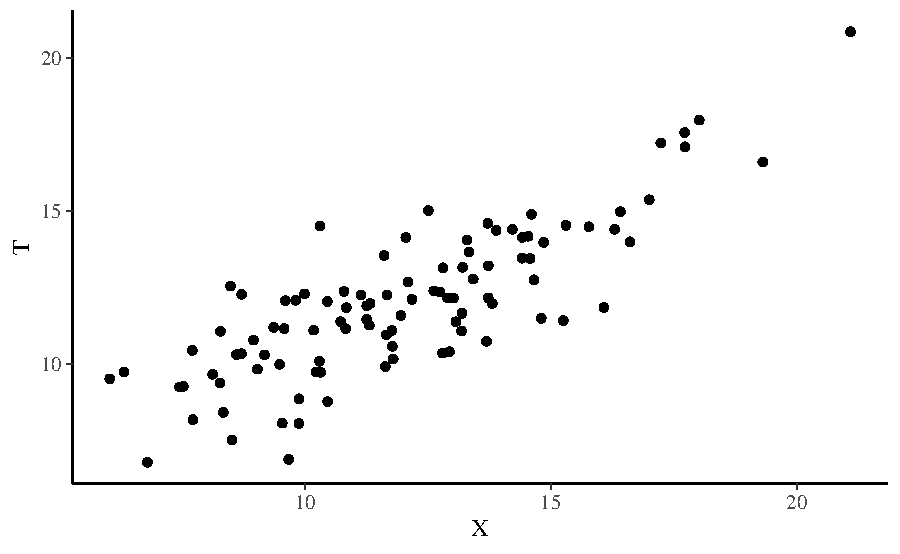
\includegraphics{cvsm22_files/figure-latex/unnamed-chunk-8-1} 

}

\caption{Simulazione della relazione tra punteggio osservato e punteggio vero per 100 individui in base alle assunzioni della CTT.}\label{fig:unnamed-chunk-8}
\end{figure}

Secondo la CTT, il valore atteso di \(T\) è uguale al valore atteso di \(X\). Verifichiamo questa assunzione della CTT nei nostri dati:

\begin{Shaded}
\begin{Highlighting}[]
\FunctionTok{mean}\NormalTok{(T)}
\CommentTok{\#\textgreater{} [1] 12}
\FunctionTok{mean}\NormalTok{(X)}
\CommentTok{\#\textgreater{} [1] 12}
\end{Highlighting}
\end{Shaded}

L'errore deve avere media zero, varianza \(\sigma_E^2\) e deve essere incorrelato con \(T\):

\begin{Shaded}
\begin{Highlighting}[]
\FunctionTok{mean}\NormalTok{(E)}
\CommentTok{\#\textgreater{} [1] 4.061e{-}18}
\FunctionTok{var}\NormalTok{(E)}
\CommentTok{\#\textgreater{} [1] 3}
\FunctionTok{cor}\NormalTok{(T, E)}
\CommentTok{\#\textgreater{} [1] {-}1.947e{-}16}
\end{Highlighting}
\end{Shaded}

Ricordiamo che la radice quadrata della varianza degli errori è chiamata errore standard della misurazione, \(\sigma_E\). La quantità \(\sqrt{\sigma_E^2}\) fornisce una misura della dispersione del punteggio osservato attorno al valore vero, nella condizione ipotetica di effettuare ripetute somministrazioni del test.

\begin{Shaded}
\begin{Highlighting}[]
\FunctionTok{sqrt}\NormalTok{(}\DecValTok{3}\NormalTok{)}
\CommentTok{\#\textgreater{} [1] 1.732}
\end{Highlighting}
\end{Shaded}

Dato che \(T\) e \(E\) sono incorrelati, ne segue che la varianza del punteggio osservato \(X\) è uguale alla somma della varianza del punteggio vero \(T\) e della varianza degli errori \(E\):

\begin{Shaded}
\begin{Highlighting}[]
\FunctionTok{var}\NormalTok{(X)}
\CommentTok{\#\textgreater{} [1] 9}
\FunctionTok{var}\NormalTok{(T) }\SpecialCharTok{+} \FunctionTok{var}\NormalTok{(E)}
\CommentTok{\#\textgreater{} [1] 9}
\end{Highlighting}
\end{Shaded}

La varianza del punteggio vero \(T\) è uguale alla covarianza tra il punteggio vero \(T\) e il punteggio osservato \(X\):

\begin{Shaded}
\begin{Highlighting}[]
\FunctionTok{cov}\NormalTok{(T, X)}
\CommentTok{\#\textgreater{} [1] 6}
\FunctionTok{var}\NormalTok{(T)}
\CommentTok{\#\textgreater{} [1] 6}
\end{Highlighting}
\end{Shaded}

La correlazione tra il punteggio osservato e il punteggio vero è uguale al rapporto tra la deviazione standard del punteggio vero e la deviazione standard del punteggio osservato:

\begin{Shaded}
\begin{Highlighting}[]
\FunctionTok{cor}\NormalTok{(X, T)}
\CommentTok{\#\textgreater{} [1] 0.8165}
\FunctionTok{sd}\NormalTok{(T) }\SpecialCharTok{/} \FunctionTok{sd}\NormalTok{(X)}
\CommentTok{\#\textgreater{} [1] 0.8165}
\end{Highlighting}
\end{Shaded}

Focalizziamoci ora sull'attendibiiltà. Per la CTT, l'attendibilità è uguale al quadrato del coefficiente di correlazione tra il punteggio vero \(T\) e il punteggio osservato \(X\):

\begin{Shaded}
\begin{Highlighting}[]
\FunctionTok{cor}\NormalTok{(X, T)}\SpecialCharTok{\^{}}\DecValTok{2}
\CommentTok{\#\textgreater{} [1] 0.6667}
\end{Highlighting}
\end{Shaded}

La motivazione di questa simulazione è quella di mettere in relazione il coefficiente di attendibilità, calcolato con le formule della CTT, con il modello di regressione lineare. Analizziamo dunque i dati della simulazione mediante il seguente modello di regressione lineare:

\[
X = a + b T + E
\]

\begin{Shaded}
\begin{Highlighting}[]
\NormalTok{fm }\OtherTok{\textless{}{-}} \FunctionTok{lm}\NormalTok{(X }\SpecialCharTok{\textasciitilde{}}\NormalTok{ T)}
\FunctionTok{summary}\NormalTok{(fm)}
\CommentTok{\#\textgreater{} }
\CommentTok{\#\textgreater{} Call:}
\CommentTok{\#\textgreater{} lm(formula = X \textasciitilde{} T)}
\CommentTok{\#\textgreater{} }
\CommentTok{\#\textgreater{} Residuals:}
\CommentTok{\#\textgreater{}    Min     1Q Median     3Q    Max }
\CommentTok{\#\textgreater{} {-}4.197 {-}1.101  0.052  1.155  4.239 }
\CommentTok{\#\textgreater{} }
\CommentTok{\#\textgreater{} Coefficients:}
\CommentTok{\#\textgreater{}             Estimate Std. Error t value Pr(\textgreater{}|t|)    }
\CommentTok{\#\textgreater{} (Intercept) 8.53e{-}15   8.75e{-}01       0        1    }
\CommentTok{\#\textgreater{} T           1.00e+00   7.14e{-}02      14   \textless{}2e{-}16 ***}
\CommentTok{\#\textgreater{} {-}{-}{-}}
\CommentTok{\#\textgreater{} Signif. codes:  }
\CommentTok{\#\textgreater{} 0 \textquotesingle{}***\textquotesingle{} 0.001 \textquotesingle{}**\textquotesingle{} 0.01 \textquotesingle{}*\textquotesingle{} 0.05 \textquotesingle{}.\textquotesingle{} 0.1 \textquotesingle{} \textquotesingle{} 1}
\CommentTok{\#\textgreater{} }
\CommentTok{\#\textgreater{} Residual standard error: 1.74 on 98 degrees of freedom}
\CommentTok{\#\textgreater{} Multiple R{-}squared:  0.667,  Adjusted R{-}squared:  0.663 }
\CommentTok{\#\textgreater{} F{-}statistic:  196 on 1 and 98 DF,  p{-}value: \textless{}2e{-}16}
\end{Highlighting}
\end{Shaded}

Si noti che la retta di regressione ha intercetta 0 e pendenza 1. Questo è coerente con l'assunzione \(\E(X) = \E(T)\). Ma il risultato più importante di questa simulazione è il seguente: il coefficiente di determinazione (\(R^2\) = 0.67) del modello di regressione \(X = 0 + 1 \times T + E\) è identico al coefficiente di attendibilità che abbiamo calcolato con la formula \(\rho_{XT}^2 = \frac{\sigma_{T}^2}{\sigma_X^2}\):

\begin{Shaded}
\begin{Highlighting}[]
\FunctionTok{var}\NormalTok{(T) }\SpecialCharTok{/} \FunctionTok{var}\NormalTok{(X)}
\CommentTok{\#\textgreater{} [1] 0.6667}
\end{Highlighting}
\end{Shaded}

Ciò ci consente di attribuire al coefficiente di attendibilità la seguente interpretazione: l'attendibilità di un test non è altro che la quota di varianza del punteggio osservato \(X\) che viene spiegata dalla regressione di \(X\) sul punteggio vero \(T\) in un modello di regressione dove \(\alpha\) = 0 e \(\beta\) = 1.

Che cosa si può concludere dai risultati di questa simulazione? Possiamo dire che, in base alla CTT,

\begin{itemize}
\tightlist
\item
  c'è una relazione lineare tra il punteggio osservato \(X\) e il punteggio vero \(T\); tale relazione lineare ha pendenza unitaria e intercetta zero.
\item
  La CTT fa proprie le assunzioni del modello di regressione lineare: incorrelazione tra variabile esplicativa \(T\) ed errore \(E\), e indipendenza e gaussianità degli errori.
\item
  Come conseguenza di tali assunzioni, il coefficiente di attendibilità non è altro che la quota di varianza del punteggio osservato \(X\) che viene spiegata dal punteggio vero tramite una regressione lineare, ovvero non è altro che il coefficiente di determinazione del modello di regressione \(X = \alpha + \beta T + E,\) dove \(\alpha\) = 0 e \(\beta\) = 1.
\end{itemize}

Vedremo in seguito come sia possibile formulare la CTT nei termini del modello statistico dell'analisi fattoriale. Nel linguaggio dell'analisi fattoriale, la varianza dell'errore \(\sigma^2_E\) viene chiamata \emph{specificità} (\emph{uniqueness}).

\hypertarget{misurazioni-parallele-e-affidabilituxe0}{%
\section{Misurazioni parallele e affidabilità}\label{misurazioni-parallele-e-affidabilituxe0}}

L'equazione \(\rho_{XT}^2 = \frac{\sigma_{T}^2}{\sigma_X^2}\) definisce il coefficiente di attendibilità ma non fornisce gli strumenti per calcolarlo, dato che la varianza del punteggio vero \(\sigma_{T}^2\) è una quantità incognita. Il metodo utilizzato dalla CTT per ottenere una stima (empirica) dell'attendibilità è quello delle forme parallele del test. Se è possibile elaborare versioni alternative dello stesso test che risultino equivalenti tra loro in termini di contenuto, modalità di risposta e caratteristiche statistiche, allora diventa anche possibile stimare il coefficiente di attendibilità.

Secondo la CTT, due test \(X=T+E\) e \(X^\prime=T^\prime+E^\prime\) si dicono misurazioni parallele della stessa abilità latente se il punteggio vero \(T\) è uguale al punteggio vero \(T^\prime\) e se la varianza degli errori \(\V(E)\) è uguale alla varianza degli errori \(\V(E^\prime)\).

Se il punteggio vero è uguale al valore atteso del punteggio osservato, \(T = \E(X)\), allora devono essere uguali anche le medie dei punteggi osservati delle due forme parallele del test, \(\E(X) = \E(X^\prime)\).

\begin{proof}
Consideriamo l'eguaglianza dei valori attesi dei punteggi osservati in due forme parallele del test: \(\E(X) = \E(X^\prime)\). Risulta immediato che

\[
\E(X) = \E(T + E) = \E(T) + \E(E) = T,
\]

dato che \(\E(E)=0\) e \(T\) non è una variabile aleatoria. Inoltre, \(\E(X^\prime)=T\), dato che \(T=T^\prime\). Ne segue che \(\E(X) =\E(X^\prime)\).
\end{proof}

In maniera corrispondente, anche le varianze dei punteggi osservati di due misurazioni parallele devono essere uguali, \(\V(X) = \V(X^\prime)\).

\begin{proof}
Per la misurazione parallela \(X\) abbiamo

\[
\V(X) = \V(T + E)=  \V(T) +  \V(E);
\]

per la misurazione parallela \(X^\prime\) abbiamo

\[
\V(X^\prime) = \V(T^\prime + E^\prime) =  \V(T^\prime) +  \V(E^\prime).
\]

Dato che \(\V(E)=\V(E^\prime)\) e che \(T=T^\prime\), ne segue che \(\V(X) =\V(X^\prime)\).
\end{proof}

Per costruzione, inoltre, gli errori \(E\) e \(E^\prime\) devono essere incorrelati con \(T\) e tra loro.

\hypertarget{la-correlazione-tra-misurazioni-parallele}{%
\subsection{La correlazione tra misurazioni parallele}\label{la-correlazione-tra-misurazioni-parallele}}

Un'ulteriore assunzione della CTT è la seguente. La CTT assume che, data una serie di misurazioni parallele \(X_1, X_2, X_3, \dots\) e un arbitrario test \(Z\), si ha

\[
\rho(X_1, X_2) = \rho(X_1, X_3) = \rho(X_2, X_3) = \dots
\]

e

\[
\rho(X_1, Z) = \rho(X_2,Z) = \rho(X_3, Z) = \dots
\]

ovvero, tutte le misurazioni parallele sono correlate tra loro nella stessa misura e ciascuna misurazione parallela correla nella stessa misura con qualunque altro test.

L'assunzione precedente può essere espressa, in maniera equivalente, come segue. Si consideri la matrice di correlazioni calcolata su tutto il dominio degli item (ovvero, la matrice delle correlazioni tra ciascuna coppia di item nel dominio del costrutto). La correlazione media di questa matrice quantifica la capacità media di ciascun item di rappresentare il costrutto. La CTT assume che la correlazione di ciascun item con ciascuno degli altri sia costante (ovvero, uguale per qualunque coppia di item). Detto in altri termini: secondo la CTT ciascun item rappresenta il costrutto nella stessa misura. Questa è un'assunzione molto forte che si riflette, come vedremo, nella formula del coefficiente \(\alpha\) di Cronbach utilizzata per misurare l'attendibilità come consistenza interna. È un'assunzione molto forte che raramente viene soddisfatta in pratica.

Secondo la CTT, dunque, forme parallele del test devono avere lo stesso valore atteso e la stessa varianza. Inoltre, ciascuna forma parallela deve correlare nella stessa misura con qualunque altro test. In che modo si differenziano allora le forme parallele del test? L'unica differenza tra le forme parallele del test riguarda il punteggio osservato: a causa dell'errore di misurazione \(X \neq X^\prime\).

Il concetto di forme parallele del test è estremamente importante per la CTT perché attraverso tale nozione diventa possibile giungere ad una stima empirica dell'attendibilità. Prima di presentare questo ultimo passaggio algebrico è però necessario calcolare la correlazione tra due misurazioni parallele.

\hypertarget{la-correlazione-tra-due-forme-parallele-del-test}{%
\subsection{La correlazione tra due forme parallele del test}\label{la-correlazione-tra-due-forme-parallele-del-test}}

Secondo la CTT, la correlazione tra due misurazioni parallele è uguale al rapporto tra la varianza del punteggio vero e la varianza del punteggio osservato. Ricordiamo che la varianza del punteggio osservato è uguale nelle due forme parallele del test: \(\V(X) = \V(X^\prime)\).

\begin{proof}
Assumendo, senza perdita di generalità, che \(\E(X)=\E(X')=\E(T)=0\), possiamo scrivere

\begin{equation}
\begin{aligned}
\rho_{X X^\prime} &= \frac{\sigma(X, X^\prime)}{\sigma(X) \sigma(X^\prime)}\notag\\
&= \frac{\E(XX^\prime)}{\sigma(X) \sigma(X^\prime)}\notag\\
&=\frac{\E[(T+E)(T+E^\prime)]}{\sigma(X) \sigma(X^\prime)}\notag\\
&=\frac{\E(T^2)+\E(TE^\prime)+\E(TE)+ \E(EE^\prime)}{\sigma(X) \sigma(X^\prime)}.\notag
\end{aligned}
\end{equation}

Ma \(\E(TE) = \E(TE^\prime) = \E(EE^\prime)=0\); inoltre, \(\sigma(X) =\sigma(X^\prime)= \sigma_X\). Dunque,

\begin{equation}
\rho_{X X^\prime} =\frac{\E(T^2)}{\sigma_X \sigma_X} = \frac{\sigma^2_T}{\sigma^2_X}.
\label{eq:3-3-5}
\end{equation}
\end{proof}

Si noti come la \eqref{eq:3-3-5} e l'equazione che definisce il coefficiente di attendibilità, ovvero \(\rho_{XT}^2 = \frac{\sigma_{T}^2}{\sigma_X^2}\), riportano tutte e due la stessa quantità a destra dell'uguale. Otteniamo così un importante risultato. Il coefficiente di attendibilità, ovvero il quadrato del coefficiente di correlazione tra il punteggio osservato e il punteggio vero, è uguale alla correlazione tra il valore osservato di due misurazioni parallele:

\begin{equation}
\rho^2_{XT} =  \rho_{XX^\prime}.
\label{eq:rho2xt-rhoxx}
\end{equation}

Tale risultato è importante perché consente di esprimere la quantità inosservabile \(\rho^2_{XT}\) nei termini della quantità \(\rho_{XX^\prime}\) che può essere calcolata sulla base del punteggio osservato. Quindi, la stima di \(\rho^2_{XT}\) si riduce alla stima di \(\rho^2_{XX^\prime}\). Per questa ragione, la \eqref{eq:rho2xt-rhoxx} è forse la formula più importante della CTT.

\hypertarget{la-correlazione-tra-punteggio-osservato-e-punteggio-vero}{%
\subsection{La correlazione tra punteggio osservato e punteggio vero}\label{la-correlazione-tra-punteggio-osservato-e-punteggio-vero}}

Consideriamo ora la correlazione tra punteggio osservato e punteggio vero. La \eqref{eq:rho2xt-rhoxx} si può scrivere come

\[
\rho_{XT} = \sqrt{\rho_{XX^\prime}}.
\]

Tale risultato si può interpretare dicendo che la correlazione tra punteggio osservato e punteggio vero è uguale alla radice quadrata del coefficiente di attendibilità.

\hypertarget{i-fattori-che-influenzano-lattendibilituxe0}{%
\subsection{I fattori che influenzano l'attendibilità}\label{i-fattori-che-influenzano-lattendibilituxe0}}

Considerando le precedenti tre equazioni

\[
\rho^2_{XT} = \rho_{XX'},\quad
\rho_{XT}^2 = \frac{\sigma_{T}^2}{\sigma_X^2}, \quad
\rho_{XT}^2 = 1-\frac{\sigma_{E}^2}{\sigma_X^2},
\]

possiamo dire che ci sono tre modi equivalenti per concludere che l'attendibilità di un test è alta. L'attendibilità di un test è alta

\begin{enumerate}
\def\labelenumi{\arabic{enumi}.}
\tightlist
\item
  quando la correlazione tra misurazioni parallele è alta,
\item
  quando la varianza del punteggio vero è grande relativamente alla varianza del punteggio osservato,
\item
  quando la varianza dell'errore di misura è piccola relativamente alla varianza del punteggio osservato.
\end{enumerate}

Tali considerazioni hanno importanti implicazioni per le scelte che devono guidare la costruzione di un test. Si consideri, in particolare, l'equazione \(\rho^2_{XT} = \rho_{XX'}\). Se interpretiamo \(\rho_{XX'}\) come la correlazione tra due item, allora tale equazione ci fornisce un criterio per la scelta degli item da includere in un test: dobbiamo includere nel test gli item che correlano maggiormente tra loro. In questo modo, infatti, l'attendibilità del test aumenterà perché gli item inclusi nel test risultano maggiormente correlati con il punteggio vero.

\hypertarget{metodi-alternativi-per-la-stima-del-coefficiente-di-attendibilituxe0}{%
\section{Metodi alternativi per la stima del coefficiente di attendibilità}\label{metodi-alternativi-per-la-stima-del-coefficiente-di-attendibilituxe0}}

Come si stima in pratica l'affidabilità? Un modo grossolano (e molto impreciso) consiste nel somministrare allo stesso gruppo di individui lo stesso test in due differenti momenti e di calcolare il coefficiente di correlazione dei punteggi totali (\emph{test-retest reliability}). \citet{mcdonald2013test} afferma che tale procedura può essere giustificata in due modi diversi. La prima giustificazione è basata sull'assunzione che il valore vero non varia tra le due somministrazioni del test. Se le cose stanno in questo modo, gli errori saranno indipendenti e la correlazione tra il punteggio osservato nelle due somministrazioni ci fornirà una stima di \(\rho_{XX^\prime}\). Il problema è che non disponiamo di nessuno strumento per distinguere questa situazione ideale dal caso in cui viene violata l'assunzione dell'invarianza del punteggio vero. Una seconda giustificazione del metodo test-retest ci porta a definire il punteggio vero di retest come la componente del punteggio osservato che non varia tra le due somministrazioni. Il tal senso, il coefficiente di attendibilità viene concepito come un coefficiente di stabilità temporale. In generale, maggiore è l'intervallo temporale tra le due somministrazioni, minore sarà il valore del coefficiente di stabilità temporale. Uno dei problemi del metodo test-retest è che due somministrazioni successive di un test ci forniscono soltanto un sottoinsieme delle possibili informazioni che verrebbero raccolte da uno studio longitudinale che copre un periodo temporale maggiore. Se tale studio longitudinale venisse eseguito, potremmo trovare la funzione che descrive la variazione del punteggio osservato in funzione del tempo. In generale, tale funzione non può essere descritta da un singolo parametro. Resta aperta la domanda di quale sia relazione tra questa funzione e il coefficiente di attendibilità.

Se sono disponibili due forme parallele dello stesso test, l'affidabilità può essere calcolata mediante il coefficiente di correlazione dei punteggi totali dei due test (\emph{parallel-forms reliability}), valendo l'uguaglianza \(\rho_{XX^\prime} = \rho^2_{XT}\). Anche questo metodo, come il metodo del test-retest, non è esente da errori.

Il metodo di stima più diffuso è quello conosciuto come Cronbach's alpha (\emph{internal consistency reliability}) originariamente ricavato da \citet{kuder1937theory} per item dicotomici e poi generalizzato da \citet{cronbach1951coefficient} per item a risposte ordinali di qualunque tipo. L'idea su cui si basa consiste nel fatto che ogni singolo item del test, se confrontato con tutti gli altri, può essere usato per stimarne l'affidabilità. L'analisi degli item viene utilizzata per ottenere una stima della consistenza interna del test e valuta la misura in cui gli item del test sono espressione dello stesso costrutto.

\hypertarget{ch:growth_models}{%
\chapter{Curve di crescita latente}\label{ch:growth_models}}

\hypertarget{dati-longitudinali}{%
\section{Dati longitudinali}\label{dati-longitudinali}}

Un importante classe di modelli a variabili latenti è quella dei modelli delle curve di crescita latente (\emph{latent growth models}, LGM). I modelli delle curve di crescita latente vengono spesso utilizzati per analizzare dati longitudinali. In questo tipo di dati, una misura di esito viene ottenuta in diversi momenti del tempo e si vuole studiare il cambiamento nel tempo. In molti casi, la traiettoria nel tempo può essere modellata come una semplice funzione lineare o quadratica. Le differenze individuali vengono catturate dagli \emph{effetti random} che sono convenientemente rappresentati da variabili latenti (continue), spesso chiamate \emph{fattori di crescita} (\emph{growth factors}).

Possiamo pensare ai modelli LGM come ad un'estensione del modello CFA dotato di \texttt{meanstructure}. L'inclusione della \texttt{meanstructure} significa che non possiamo usare in input la matrice di covarianza campionaria, ma dobbiamo invece utilizzare i dati grezzi (ovvero, le singole osservazioni per ciascun parecipante). Un'altro requisito degli LGM è che i dati devono essere forniti del formato \texttt{wide}, il che significa che ogni colonna rappresenta la variabile di esito in un diverso momento nel tempo. Si presume che ogni osservazione o riga sia indipendente dalle altre; le colonne motrano invece una dipendenza temporale tra loro.

I modelli LGM sono un caso speciale di CFA e corrispondono un modello CFA a due fattori in cui le saturazioni fattoriali sono fissate a valori predefiniti. Nello specifico, le saturazioni sul fattore che specifica le intercette delle funzioni individuali di crescita sono tutte fissate a 1; le saturazioni sul fattore che specifica le pendenze delle funzioni individuali di crescita sono fissate in modo tale da corrispondere ai diversi momenti del tempo, laddove la saturazione in corrispondenza del momento \(t_0\) è uguale a 0 e la progressione procede con incrementi di 1 (ovvvero, \(0, 1, \dots, t-1\)).

Si giunge così alla seguente specifiazione del modello fattoriale:

\begin{equation}
y_{it} = \tau_i + (1) \xi_1 + (t) \xi_2 + \delta_t,
\end{equation}

con \(t = 0, 1, 2, 3\) nel caso di quattro misurazioni temporali. Si noti che, per disegno, \(\tau_i = 0\).

\hypertarget{un-esempio-concreto}{%
\subsection{Un esempio concreto}\label{un-esempio-concreto}}

L'esempio che discuteremo utilizza i dati di un tutorial \texttt{lavaan}, ovvero un campione di dati artificiali chiamato \texttt{Demo.growth} in cui un punteggio viene misurato su quattro punti temporali. I dati sono i seguenti:

\begin{Shaded}
\begin{Highlighting}[]
\FunctionTok{data}\NormalTok{(Demo.growth)}
\FunctionTok{glimpse}\NormalTok{(Demo.growth)}
\CommentTok{\#\textgreater{} Rows: 400}
\CommentTok{\#\textgreater{} Columns: 10}
\CommentTok{\#\textgreater{} $ t1 \textless{}dbl\textgreater{} 1.7256, {-}1.9842, 0.3195, 0.7769, 0.4489, {-}\textasciitilde{}}
\CommentTok{\#\textgreater{} $ t2 \textless{}dbl\textgreater{} 2.1424, {-}4.4006, {-}1.2691, 3.5314, {-}0.7728,\textasciitilde{}}
\CommentTok{\#\textgreater{} $ t3 \textless{}dbl\textgreater{} 2.7732, {-}6.0166, 1.5600, 3.1382, {-}1.5035, \textasciitilde{}}
\CommentTok{\#\textgreater{} $ t4 \textless{}dbl\textgreater{} 2.51596, {-}7.02962, 2.86853, 5.36374, 0.078\textasciitilde{}}
\CommentTok{\#\textgreater{} $ x1 \textless{}dbl\textgreater{} {-}1.1641, {-}1.7454, 0.9202, 2.3595, {-}1.0887,\textasciitilde{}}
\CommentTok{\#\textgreater{} $ x2 \textless{}dbl\textgreater{} 0.1742, {-}1.5769, {-}0.1418, 0.7080, {-}1.0100,\textasciitilde{}}
\CommentTok{\#\textgreater{} $ c1 \textless{}dbl\textgreater{} {-}0.02768, {-}2.03197, 0.05237, 0.01911, 0.65\textasciitilde{}}
\CommentTok{\#\textgreater{} $ c2 \textless{}dbl\textgreater{} 0.55492, 0.12533, {-}1.25774, 0.64738, 0.730\textasciitilde{}}
\CommentTok{\#\textgreater{} $ c3 \textless{}dbl\textgreater{} 0.25448, {-}1.56423, {-}1.80339, {-}0.43238, {-}0.\textasciitilde{}}
\CommentTok{\#\textgreater{} $ c4 \textless{}dbl\textgreater{} {-}1.00640, 1.22927, {-}0.32726, {-}1.03240, {-}0.\textasciitilde{}}
\end{Highlighting}
\end{Shaded}

La variabile dipendente è rappresentata dalle quattro colonne chiamate \texttt{t1}, \texttt{t2}, \texttt{t3} e \texttt{t4} che corrispondono alla serie temporale con quattro misurazioni per ciascun soggetto.

Trasformiamo i dati in formato \texttt{long}:

\begin{Shaded}
\begin{Highlighting}[]
\NormalTok{demo\_growth\_long }\OtherTok{\textless{}{-}}\NormalTok{ Demo.growth }\SpecialCharTok{\%\textgreater{}\%}
\NormalTok{  dplyr}\SpecialCharTok{::}\FunctionTok{select}\NormalTok{(t1, t2, t3, t4) }\SpecialCharTok{\%\textgreater{}\%}
  \FunctionTok{pivot\_longer}\NormalTok{(}
    \AttributeTok{cols =} \FunctionTok{starts\_with}\NormalTok{(}\StringTok{"t"}\NormalTok{),}
    \AttributeTok{names\_to =} \StringTok{"t"}\NormalTok{,}
    \AttributeTok{values\_to =} \StringTok{"y"}
\NormalTok{  ) }\SpecialCharTok{\%\textgreater{}\%}
  \FunctionTok{as.data.frame}\NormalTok{()}
\NormalTok{demo\_growth\_long}\SpecialCharTok{$}\NormalTok{time }\OtherTok{\textless{}{-}} \FunctionTok{rep}\NormalTok{(}\DecValTok{0}\SpecialCharTok{:}\DecValTok{3}\NormalTok{, }\DecValTok{400}\NormalTok{)}
\NormalTok{demo\_growth\_long}\SpecialCharTok{$}\NormalTok{id }\OtherTok{\textless{}{-}} \FunctionTok{rep}\NormalTok{(}\DecValTok{1}\SpecialCharTok{:}\DecValTok{400}\NormalTok{, }\AttributeTok{each =} \DecValTok{4}\NormalTok{)}
\end{Highlighting}
\end{Shaded}

Esaminiamo un campione casuale di 9 soggetti. È presente una notevole variazione da soggetto a soggetto:

\begin{Shaded}
\begin{Highlighting}[]
\NormalTok{id\_sel }\OtherTok{\textless{}{-}} \FunctionTok{sample}\NormalTok{(}\DecValTok{1}\SpecialCharTok{:}\DecValTok{400}\NormalTok{, }\DecValTok{9}\NormalTok{)}
\NormalTok{d }\OtherTok{\textless{}{-}}\NormalTok{ demo\_growth\_long[demo\_growth\_long}\SpecialCharTok{$}\NormalTok{id }\SpecialCharTok{\%in\%}\NormalTok{ id\_sel, ]}
\NormalTok{d }\SpecialCharTok{\%\textgreater{}\%}
  \FunctionTok{ggplot}\NormalTok{(}\FunctionTok{aes}\NormalTok{(}\AttributeTok{x =}\NormalTok{ time, }\AttributeTok{y =}\NormalTok{ y)) }\SpecialCharTok{+}
  \FunctionTok{geom\_line}\NormalTok{() }\SpecialCharTok{+}
  \FunctionTok{facet\_wrap}\NormalTok{(}\SpecialCharTok{\textasciitilde{}}\NormalTok{id)}
\end{Highlighting}
\end{Shaded}

\begin{center}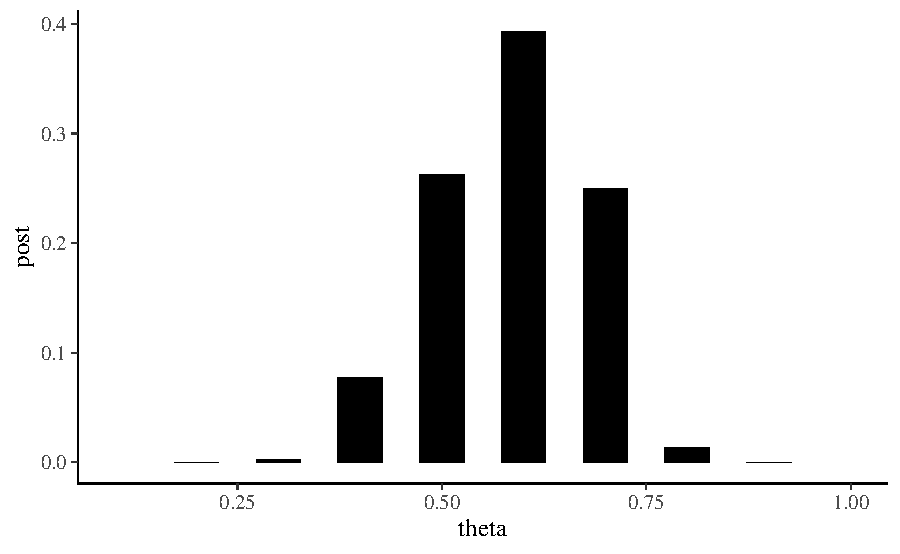
\includegraphics{cvsm22_files/figure-latex/unnamed-chunk-21-1} \end{center}

Notiamo che un semplce modello lineare è appropriato per rendere conto della variazione temporale della variabile risposta:

\begin{Shaded}
\begin{Highlighting}[]
\NormalTok{d }\SpecialCharTok{\%\textgreater{}\%}
  \FunctionTok{ggplot}\NormalTok{(}\FunctionTok{aes}\NormalTok{(}\AttributeTok{x =}\NormalTok{ time, }\AttributeTok{y =}\NormalTok{ y)) }\SpecialCharTok{+}
  \FunctionTok{geom\_point}\NormalTok{() }\SpecialCharTok{+}
  \FunctionTok{stat\_smooth}\NormalTok{(}\AttributeTok{method =} \StringTok{"lm"}\NormalTok{, }\AttributeTok{se =} \ConstantTok{FALSE}\NormalTok{) }\SpecialCharTok{+}
  \FunctionTok{facet\_wrap}\NormalTok{(}\SpecialCharTok{\textasciitilde{}}\NormalTok{id)}
\end{Highlighting}
\end{Shaded}

\begin{center}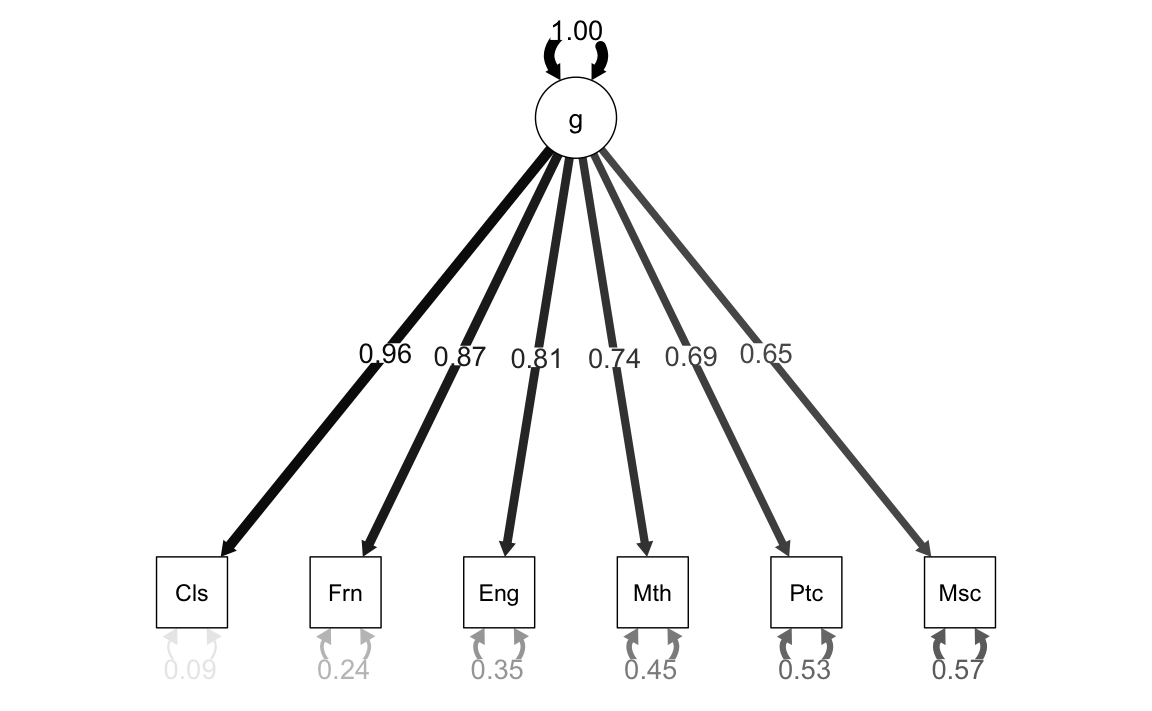
\includegraphics{cvsm22_files/figure-latex/unnamed-chunk-22-1} \end{center}

Complessivamente, i dati suggeriscono un andamento crescente della variabile risposta in funzione del tempo:

\begin{Shaded}
\begin{Highlighting}[]
\NormalTok{demo\_growth\_long }\SpecialCharTok{\%\textgreater{}\%}
  \FunctionTok{ggplot}\NormalTok{(}\FunctionTok{aes}\NormalTok{(time, y, }\AttributeTok{group =}\NormalTok{ id)) }\SpecialCharTok{+}
  \FunctionTok{geom\_line}\NormalTok{(}\AttributeTok{alpha =} \FloatTok{0.1}\NormalTok{) }\SpecialCharTok{+} \CommentTok{\# add individual line with transparency}
  \FunctionTok{stat\_summary}\NormalTok{( }\CommentTok{\# add average line}
    \FunctionTok{aes}\NormalTok{(}\AttributeTok{group =} \DecValTok{1}\NormalTok{),}
    \AttributeTok{fun =}\NormalTok{ mean,}
    \AttributeTok{geom =} \StringTok{"line"}\NormalTok{,}
    \AttributeTok{size =} \FloatTok{1.5}\NormalTok{,}
    \AttributeTok{color =} \StringTok{"black"}
\NormalTok{  ) }\SpecialCharTok{+}
  \FunctionTok{labs}\NormalTok{(}\AttributeTok{x =} \StringTok{"Time"}\NormalTok{, }\AttributeTok{y =} \StringTok{"y"}\NormalTok{)}
\end{Highlighting}
\end{Shaded}

\begin{center}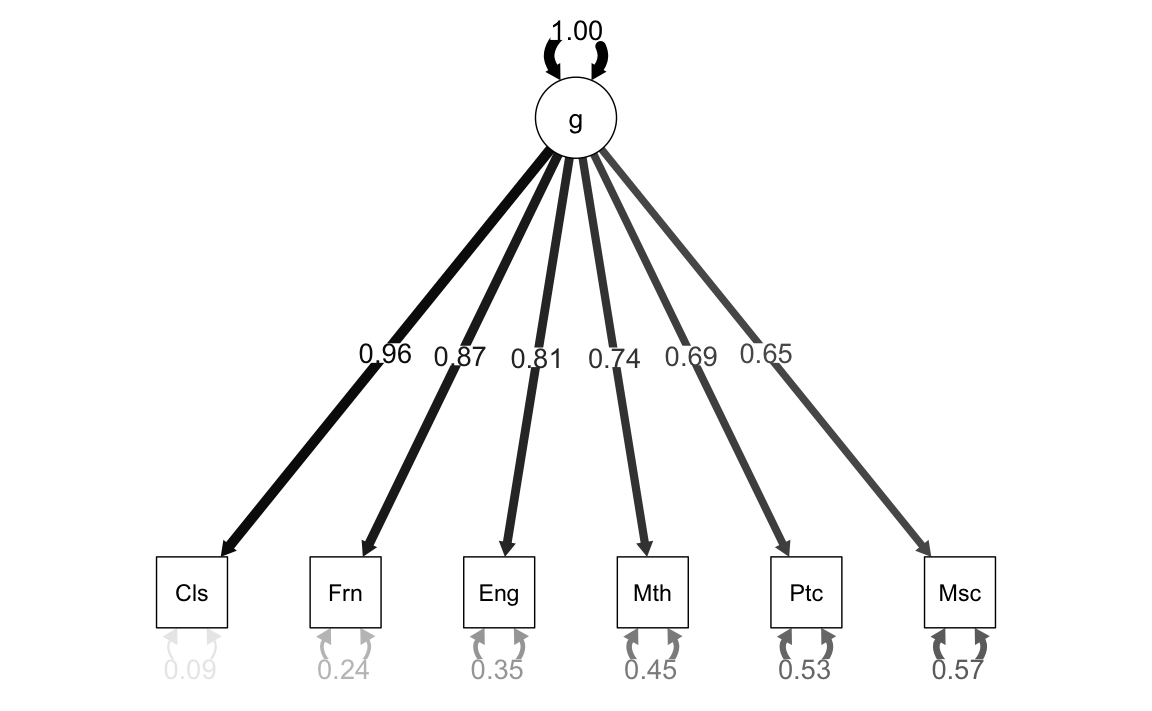
\includegraphics{cvsm22_files/figure-latex/unnamed-chunk-23-1} \end{center}

Per adattare un modello lineare di crescita a questi dati, specifichiamo il seguente modello a variabili latenti

\[
y_j = \alpha_0 + \alpha_1 \lambda_j + \zeta_{00} + \zeta_{11} \lambda_j + \epsilon_j,
\] dove

\begin{itemize}
\tightlist
\item
  \(y_j\) è la variabile di interesse che cambia nel tempo, \(j\).
\item
  \(\alpha_0\) rappresenta l'intercetta della retta di regressione al tempo \(t = 0\) (il punto di partenza della linea nera sopra).
\item
  \(\alpha_1 \lambda_j\) è il tasso medio di variazione nel tempo (la pendenza della linea nera nel grafico sopra). Qui \(\lambda_j\) è solo l'indice dei punti temporali considerati (0, 1, 2, 3).
\item
  \(\zeta_{00}\) è la varianza tra i soggetti nel punto \(t = 0\).
\item
  \(\zeta_{11} \lambda_j\) è la varianza del tasso di variazione tra i soggetti.
\item
  \(\epsilon_j\) è la varianza di ciascun soggetto attorno alla sua retta di regressione.
\end{itemize}

Tali relazioni statistiche vengono rappresentate dal modello di equazioni strutturali della figura \ref{fig:growth01}.

\begin{figure}

{\centering 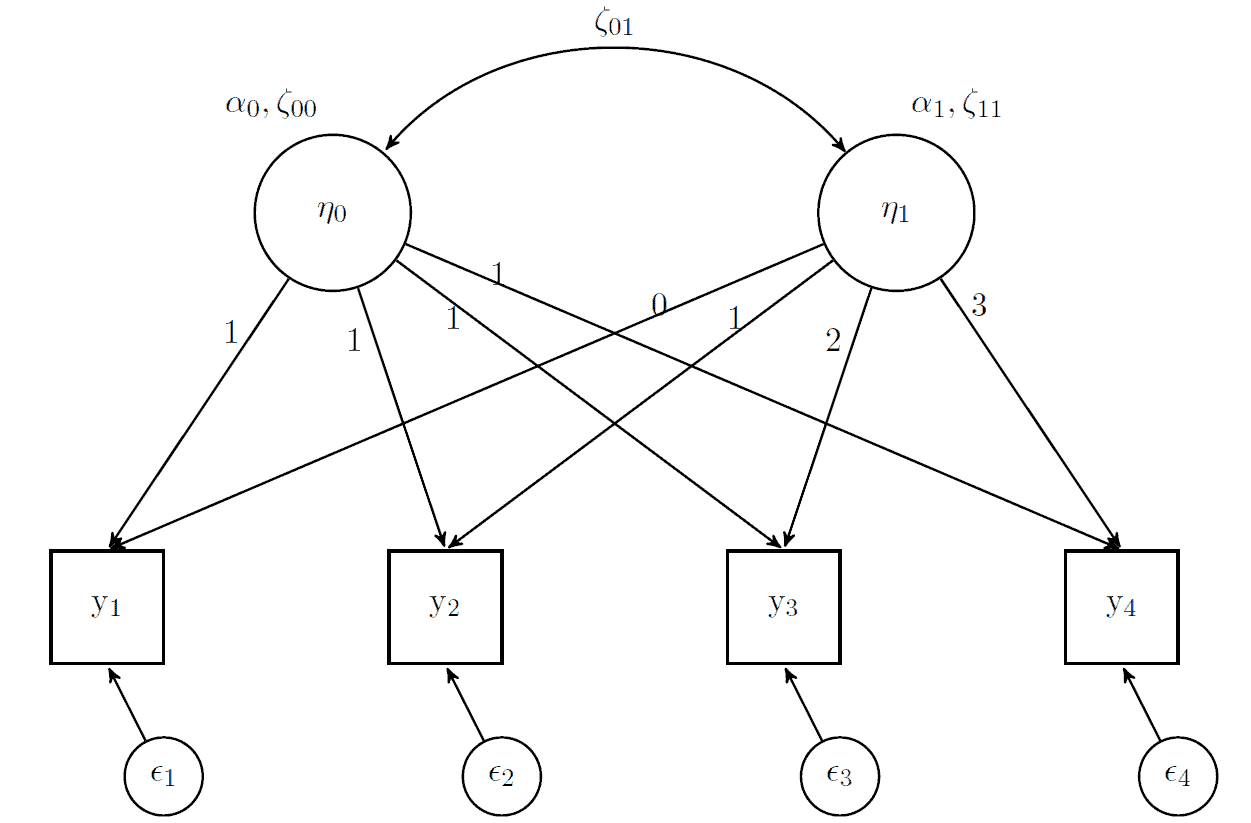
\includegraphics[width=0.9\linewidth]{images/lgm} 

}

\caption{Modello di crescita latente.}\label{fig:growth01}
\end{figure}

In altre parole, un lineare di crescita latente corrisponde ad un modello fattoriale con due variabili latenti: un fattore che corrisponde al ``punteggio vero'' delle intercette individuali e un fattore che corrisponde al ``punteggio vero'' delle pendenze individuali. Nella sitassi \texttt{lavaan} questo diventa:

\begin{Shaded}
\begin{Highlighting}[]
\NormalTok{model }\OtherTok{\textless{}{-}} \StringTok{"}
\StringTok{ i =\textasciitilde{} 1*t1 + 1*t2 + 1*t3 + 1*t4}
\StringTok{ s =\textasciitilde{} 0*t1 + 1*t2 + 2*t3 + 3*t4}
\StringTok{"}
\end{Highlighting}
\end{Shaded}

Si noti che, per il fattore \(\eta_0\) (che rappresenta le intercette), i valori delle saturazioni fattoriali sono fissate a 1 -- questo è il motivo per cui \(\alpha_0\) e \(\zeta_{00}\) compaiono da soli nell'equazione precedente: in maniera esplicita sono \(1 \cdot \alpha_0\) e \(1 \cdot \zeta_{00}\). Le saturazioni per il fattore \(\eta_1\) (che specifica le pendenze delle funzioni lineari) sono fissate ai valori dei diversi momenti nel tempo: qui i valori \(\lambda_j\) da 0 a 3. Abbiamo anche la correlazione tra \(\eta_0\) e \(\eta_1\), rappresentata dalla doppia freccia \(\zeta_{01}\). Se questo parametro è positivo, questo significa che i partecipanti tendono a diventare sempre più diversi tra loro, al passare del tempo; un'interpretazione opposta si ha se il valore del parametro è negativo.

Adattiamo il modello ai dati:

\begin{Shaded}
\begin{Highlighting}[]
\NormalTok{fit }\OtherTok{\textless{}{-}} \FunctionTok{growth}\NormalTok{(model, }\AttributeTok{data =}\NormalTok{ Demo.growth)}
\end{Highlighting}
\end{Shaded}

Esaminiamo il path diagram:

\begin{Shaded}
\begin{Highlighting}[]
\FunctionTok{semPaths}\NormalTok{(}
\NormalTok{  fit, }\StringTok{"std"}\NormalTok{,}
  \AttributeTok{posCol =} \FunctionTok{c}\NormalTok{(}\StringTok{"black"}\NormalTok{),}
  \AttributeTok{edge.label.cex =} \FloatTok{0.9}\NormalTok{,}
  \AttributeTok{sizeMan =} \DecValTok{7}\NormalTok{,}
  \AttributeTok{what =} \StringTok{"path"}
\NormalTok{)}
\end{Highlighting}
\end{Shaded}

\begin{center}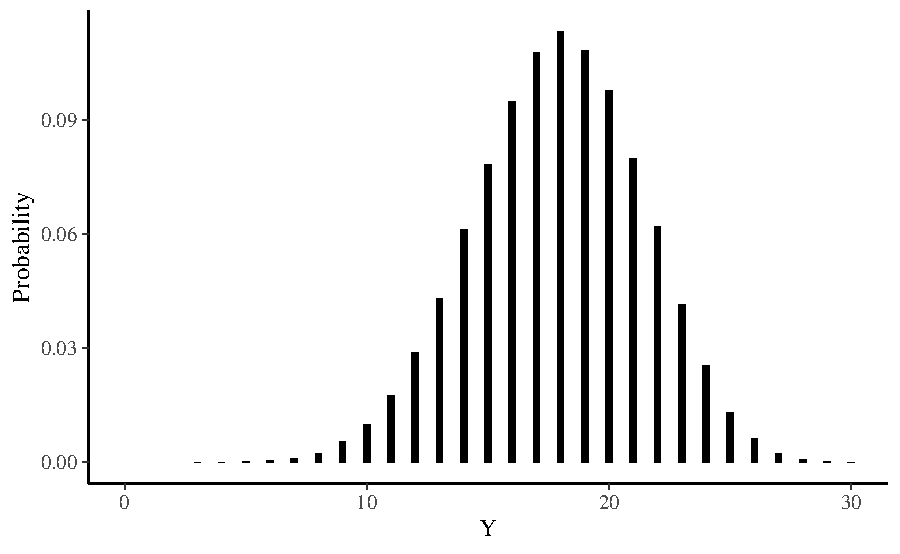
\includegraphics{cvsm22_files/figure-latex/unnamed-chunk-26-1} \end{center}

Ci sono 6 tipi di parametri di interesse:

\begin{Shaded}
\begin{Highlighting}[]
\FunctionTok{kable}\NormalTok{(}\FunctionTok{coef}\NormalTok{(fit), }\AttributeTok{booktabs =} \ConstantTok{TRUE}\NormalTok{, }\AttributeTok{format =} \StringTok{"markdown"}\NormalTok{)}
\end{Highlighting}
\end{Shaded}

\begin{longtable}[]{@{}lr@{}}
\toprule
& x \\
\midrule
\endhead
t1\textasciitilde\textasciitilde t1 & 0.5953 \\
t2\textasciitilde\textasciitilde t2 & 0.6760 \\
t3\textasciitilde\textasciitilde t3 & 0.6349 \\
t4\textasciitilde\textasciitilde t4 & 0.5076 \\
i\textasciitilde\textasciitilde i & 1.9320 \\
s\textasciitilde\textasciitilde s & 0.5869 \\
i\textasciitilde\textasciitilde s & 0.6179 \\
i\textasciitilde1 & 0.6147 \\
s\textasciitilde1 & 1.0063 \\
\bottomrule
\end{longtable}

\begin{itemize}
\tightlist
\item
  l'intercetta \(i\) = 0.615 è il valore atteso della variabile risposta al momento \(t_0\);
\item
  la pendenza \(s\) = 1.006 è il tasso di cambiamento medio della variabile risposta nel tempo. Ad ogni successivo momento temporale, il valore medio della variabile risposta aumenta in media di 1.006 punti;
\item
  varianza \(i\) = 1.932 misura la variazione tra i soggetti al momento \(t_0\) (ci dice quanto sono diverse le intercette delle rette di regressione tra i soggetti);
\item
  varianza \(s\) = 0.587 misura la variazione del tasso di crescita tra i soggetti (ci dice quanto sono diverse le pendenze delle rette di regressione tra i soggetti);
\item
  varianze \texttt{t1}, \ldots, \texttt{t4}: i valori da 0.595 a 0.508 ci dicono la variazione tra i soggetti all'interno di ciascun momento del tempo;
\item
  la covarianza tra \texttt{i} e \texttt{s} = 0.618 ci dice che i valori della variabile risposta diventano via via più diversi nel tempo tra i rispondenti (un valore negativo avrebbe l'interpretazione opposta).
\end{itemize}

Le stime dell'intercetta e della pendenza della funzione di crescita per ciascun partecipante si ottengono nel modo seguente:

\begin{Shaded}
\begin{Highlighting}[]
\NormalTok{rand\_eff }\OtherTok{\textless{}{-}} \FunctionTok{as.data.frame}\NormalTok{(}\FunctionTok{lavPredict}\NormalTok{(fit))}
\FunctionTok{head}\NormalTok{(rand\_eff)}
\CommentTok{\#\textgreater{}         i        s}
\CommentTok{\#\textgreater{} 1  1.2276  0.60278}
\CommentTok{\#\textgreater{} 2 {-}2.6796 {-}1.38498}
\CommentTok{\#\textgreater{} 3 {-}0.2955  0.88828}
\CommentTok{\#\textgreater{} 4  1.1576  1.34051}
\CommentTok{\#\textgreater{} 5 {-}0.4356  0.03193}
\CommentTok{\#\textgreater{} 6 {-}1.3122  0.50259}
\end{Highlighting}
\end{Shaded}

Le distribuzione delle stime individuali dell'intercetta e della pendenza della curva di crescita si ottengono nel modo seguente:

\begin{Shaded}
\begin{Highlighting}[]
\NormalTok{gi }\OtherTok{\textless{}{-}}\NormalTok{ rand\_eff }\SpecialCharTok{\%\textgreater{}\%}
  \FunctionTok{ggplot}\NormalTok{(}\FunctionTok{aes}\NormalTok{(}\AttributeTok{x =}\NormalTok{ i)) }\SpecialCharTok{+}
  \FunctionTok{geom\_histogram}\NormalTok{()}
\NormalTok{gh }\OtherTok{\textless{}{-}}\NormalTok{ rand\_eff }\SpecialCharTok{\%\textgreater{}\%}
  \FunctionTok{ggplot}\NormalTok{(}\FunctionTok{aes}\NormalTok{(}\AttributeTok{x =}\NormalTok{ s)) }\SpecialCharTok{+}
  \FunctionTok{geom\_histogram}\NormalTok{()}
\NormalTok{gi }\SpecialCharTok{+}\NormalTok{ gh}
\end{Highlighting}
\end{Shaded}

\begin{center}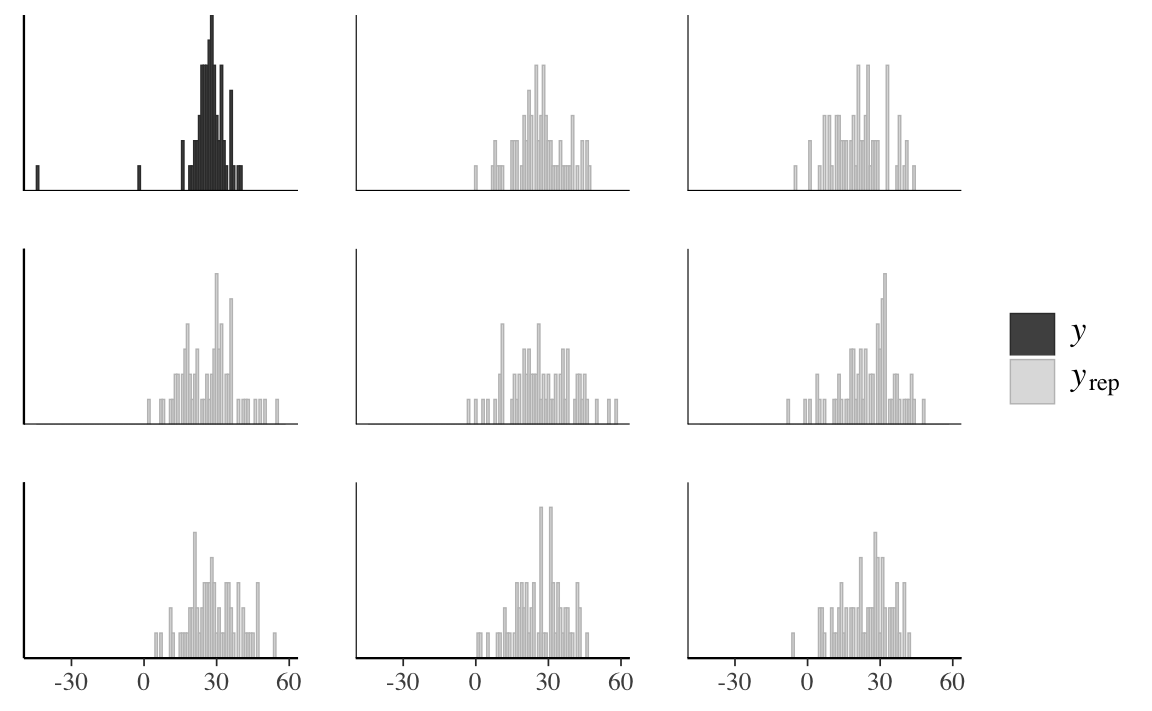
\includegraphics{cvsm22_files/figure-latex/unnamed-chunk-29-1} \end{center}

Un buon modo per capire cosa fa il modello è quello di visualizzare i punteggi previsti. Useremo qui la funzione \texttt{predict()} per salvare un nuovo oggetto con i punteggi previsti a livello individuale per l'intercetta e la pendenza;

\begin{Shaded}
\begin{Highlighting}[]
\NormalTok{pred\_lgm }\OtherTok{\textless{}{-}} \FunctionTok{predict}\NormalTok{(fit)}
\FunctionTok{head}\NormalTok{(pred\_lgm)}
\CommentTok{\#\textgreater{}            i        s}
\CommentTok{\#\textgreater{} [1,]  1.2276  0.60278}
\CommentTok{\#\textgreater{} [2,] {-}2.6796 {-}1.38498}
\CommentTok{\#\textgreater{} [3,] {-}0.2955  0.88828}
\CommentTok{\#\textgreater{} [4,]  1.1576  1.34051}
\CommentTok{\#\textgreater{} [5,] {-}0.4356  0.03193}
\CommentTok{\#\textgreater{} [6,] {-}1.3122  0.50259}
\end{Highlighting}
\end{Shaded}

Questi sono i valori previsti dal modello per ciascun partecipante. Se calcoliamo la media di queste variabili otteniamo gli stessi risultati che sono stati riportati sopra:

\begin{Shaded}
\begin{Highlighting}[]
\CommentTok{\# average of the intercepts (first column)}
\FunctionTok{mean}\NormalTok{(pred\_lgm[, }\DecValTok{1}\NormalTok{])}
\CommentTok{\#\textgreater{} [1] 0.6147}
\CommentTok{\# average of the slope (second column)}
\FunctionTok{mean}\NormalTok{(pred\_lgm[, }\DecValTok{2}\NormalTok{])}
\CommentTok{\#\textgreater{} [1] 1.006}
\end{Highlighting}
\end{Shaded}

Il cambiamento nel tempo previsto dal modello per il soggetto \(j\)-esimo è

\[
y_j = \eta_0 + \lambda_j \eta_1.
\]

Il cambiamento previsto per tutti i soggetti può essere visualizzato nel modo seguente:

\begin{Shaded}
\begin{Highlighting}[]
\CommentTok{\# create long data for each individual}
\NormalTok{pred\_lgm\_long }\OtherTok{\textless{}{-}} \FunctionTok{map}\NormalTok{(}
  \DecValTok{0}\SpecialCharTok{:}\DecValTok{3}\NormalTok{, }\CommentTok{\# loop over time}
  \ControlFlowTok{function}\NormalTok{(x) pred\_lgm[, }\DecValTok{1}\NormalTok{] }\SpecialCharTok{+}\NormalTok{ x }\SpecialCharTok{*}\NormalTok{ pred\_lgm[, }\DecValTok{2}\NormalTok{]}
\NormalTok{) }\SpecialCharTok{\%\textgreater{}\%}
  \FunctionTok{reduce}\NormalTok{(cbind) }\SpecialCharTok{\%\textgreater{}\%} \CommentTok{\# bring together the wave predictions}
  \FunctionTok{as.data.frame}\NormalTok{() }\SpecialCharTok{\%\textgreater{}\%} \CommentTok{\# make data frame}
  \FunctionTok{setNames}\NormalTok{(}\FunctionTok{str\_c}\NormalTok{(}\StringTok{"time"}\NormalTok{, }\DecValTok{0}\SpecialCharTok{:}\DecValTok{3}\NormalTok{)) }\SpecialCharTok{\%\textgreater{}\%} \CommentTok{\# give names to variables}
  \FunctionTok{mutate}\NormalTok{(}\AttributeTok{id =} \FunctionTok{row\_number}\NormalTok{()) }\SpecialCharTok{\%\textgreater{}\%} \CommentTok{\# make unique id}
  \FunctionTok{gather}\NormalTok{(}\SpecialCharTok{{-}}\NormalTok{id, }\AttributeTok{key =}\NormalTok{ time, }\AttributeTok{value =}\NormalTok{ pred) }\CommentTok{\# make long format}
\CommentTok{\# make graph}
\NormalTok{pred\_lgm\_long }\SpecialCharTok{\%\textgreater{}\%}
  \FunctionTok{ggplot}\NormalTok{(}\FunctionTok{aes}\NormalTok{(time, pred, }\AttributeTok{group =}\NormalTok{ id)) }\SpecialCharTok{+} \CommentTok{\# what variables to plot?}
  \FunctionTok{geom\_line}\NormalTok{(}\AttributeTok{alpha =} \FloatTok{0.1}\NormalTok{) }\SpecialCharTok{+} \CommentTok{\# add a transparent line for each person}
  \FunctionTok{stat\_summary}\NormalTok{( }\CommentTok{\# add average line}
    \FunctionTok{aes}\NormalTok{(}\AttributeTok{group =} \DecValTok{1}\NormalTok{),}
    \AttributeTok{fun =}\NormalTok{ mean,}
    \AttributeTok{geom =} \StringTok{"line"}\NormalTok{,}
    \AttributeTok{size =} \FloatTok{1.5}\NormalTok{,}
    \AttributeTok{color =} \StringTok{"black"}
\NormalTok{  ) }\SpecialCharTok{+}
  \FunctionTok{labs}\NormalTok{(}\AttributeTok{y =} \StringTok{"y"}\NormalTok{, }\AttributeTok{x =} \StringTok{"time"}\NormalTok{)}
\end{Highlighting}
\end{Shaded}

\begin{center}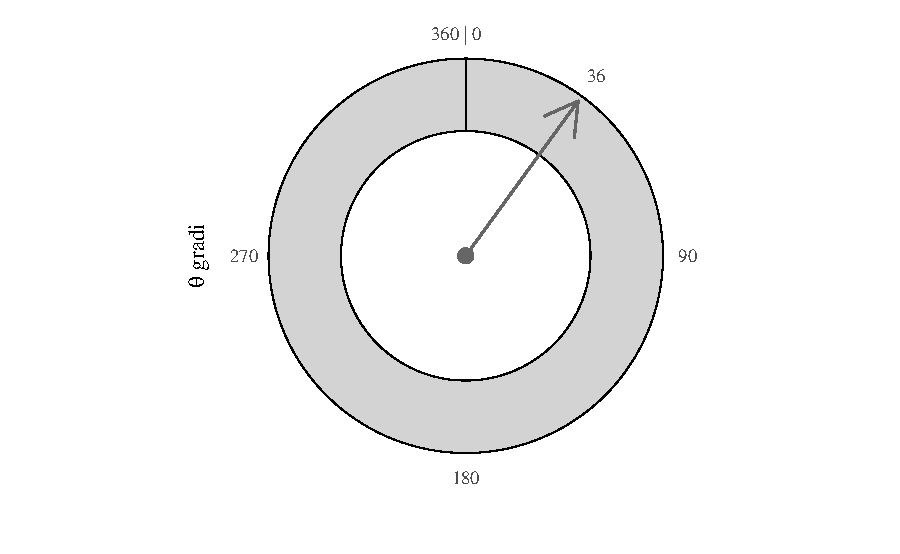
\includegraphics{cvsm22_files/figure-latex/unnamed-chunk-32-1} \end{center}

La linea nera più spessa rappresenta l'intercetta media e la pendenza media della curva di crescita del modello LGM. Ogni individuo ha una sua specifica intercetta e uno specifico tasso di cambiamento e questa diversità è catturata nelle componenti di varianza del modello

È anche possibile utilizzare le funzionalità di \texttt{lavaan} per verificare specifiche ipotesi di interesse relative ai dati longitudinali. Ad esempio, una possibile domanda riguarda l'ugualianza degli errori nel tempo. Tale domanda può essere affrontata introducendo dei vincoli nella specificazione del modello LGM e, successivamente, confrontanto la bontà dell'adattamento del modello vincolato e del modello generale.

Il modello vincolato è

\begin{Shaded}
\begin{Highlighting}[]
\NormalTok{model\_eqerr }\OtherTok{\textless{}{-}} \StringTok{"}
\StringTok{ i =\textasciitilde{} 1*t1 + 1*t2 + 1*t3 + 1*t4}
\StringTok{ s =\textasciitilde{} 0*t1 + 1*t2 + 2*t3 + 3*t4}
\StringTok{ t1 \textasciitilde{}\textasciitilde{} a*t1}
\StringTok{ t2 \textasciitilde{}\textasciitilde{} a*t2}
\StringTok{ t3 \textasciitilde{}\textasciitilde{} a*t3}
\StringTok{ t4 \textasciitilde{}\textasciitilde{} a*t4}
\StringTok{"}
\end{Highlighting}
\end{Shaded}

Adattiamo il modello vincolato:

\begin{Shaded}
\begin{Highlighting}[]
\NormalTok{fit\_eqerr }\OtherTok{\textless{}{-}} \FunctionTok{growth}\NormalTok{(model\_eqerr, }\AttributeTok{data =}\NormalTok{ Demo.growth)}
\end{Highlighting}
\end{Shaded}

Confrontiamo il modello vincolato con il modello libero:

\begin{Shaded}
\begin{Highlighting}[]
\FunctionTok{anova}\NormalTok{(fit, fit\_eqerr)}
\CommentTok{\#\textgreater{} Chi{-}Squared Difference Test}
\CommentTok{\#\textgreater{} }
\CommentTok{\#\textgreater{}           Df  AIC  BIC Chisq Chisq diff Df diff}
\CommentTok{\#\textgreater{} fit        5 5528 5564  8.07                   }
\CommentTok{\#\textgreater{} fit\_eqerr  8 5524 5548  9.68       1.61       3}
\CommentTok{\#\textgreater{}           Pr(\textgreater{}Chisq)}
\CommentTok{\#\textgreater{} fit                 }
\CommentTok{\#\textgreater{} fit\_eqerr       0.66}
\end{Highlighting}
\end{Shaded}

Il test del rapporto di verosimiglianza (\emph{likelihood ratio}) eseguito dalla funzione \texttt{anova()} produce un \(p\)-valore di 0.6573. Ciò significa che, nei dati esaminati, non si rileva una decremento della bontà dell'adattamento degna di nota nel passare dal modello libero al modello vincolato. Dunque, l'ipotesi dell'equaglianza della varianza degli errori nel tempo sembra ragionevole.

\hypertarget{un-secondo-esempio}{%
\subsection{Un secondo esempio}\label{un-secondo-esempio}}

Un modello leggermente più complesso aggiunge due regressori (\texttt{x1} e \texttt{x2}) che influenzano i fattori di crescita latenti. Inoltre, è stata aggiunta al modello una covariata \texttt{c} variabile nel tempo che influenza la misura del risultato nei quattro punti temporali.

\begin{Shaded}
\begin{Highlighting}[]
\NormalTok{model2 }\OtherTok{\textless{}{-}} \StringTok{"}
\StringTok{  \# intercept and slope with fixed coefficients}
\StringTok{    i =\textasciitilde{} 1*t1 + 1*t2 + 1*t3 + 1*t4}
\StringTok{    s =\textasciitilde{} 0*t1 + 1*t2 + 2*t3 + 3*t4}
\StringTok{  \# regressions}
\StringTok{    i \textasciitilde{} x1 + x2}
\StringTok{    s \textasciitilde{} x1 + x2}
\StringTok{  \# time{-}varying covariates}
\StringTok{    t1 \textasciitilde{} c1}
\StringTok{    t2 \textasciitilde{} c2}
\StringTok{    t3 \textasciitilde{} c3}
\StringTok{    t4 \textasciitilde{} c4}
\StringTok{"}
\end{Highlighting}
\end{Shaded}

\begin{Shaded}
\begin{Highlighting}[]
\NormalTok{fit2 }\OtherTok{\textless{}{-}} \FunctionTok{growth}\NormalTok{(model2, }\AttributeTok{data =}\NormalTok{ Demo.growth)}
\end{Highlighting}
\end{Shaded}

\begin{Shaded}
\begin{Highlighting}[]
\FunctionTok{kable}\NormalTok{(}\FunctionTok{coef}\NormalTok{(fit2), }\AttributeTok{booktabs =} \ConstantTok{TRUE}\NormalTok{, }\AttributeTok{format =} \StringTok{"markdown"}\NormalTok{)}
\end{Highlighting}
\end{Shaded}

\begin{longtable}[]{@{}lr@{}}
\toprule
& x \\
\midrule
\endhead
i\textasciitilde x1 & 0.60839 \\
i\textasciitilde x2 & 0.60411 \\
s\textasciitilde x1 & 0.26224 \\
s\textasciitilde x2 & 0.52173 \\
t1\textasciitilde c1 & 0.14336 \\
t2\textasciitilde c2 & 0.28900 \\
t3\textasciitilde c3 & 0.32754 \\
t4\textasciitilde c4 & 0.33049 \\
t1\textasciitilde\textasciitilde t1 & 0.57982 \\
t2\textasciitilde\textasciitilde t2 & 0.59559 \\
t3\textasciitilde\textasciitilde t3 & 0.48141 \\
t4\textasciitilde\textasciitilde t4 & 0.53521 \\
i\textasciitilde\textasciitilde i & 1.07946 \\
s\textasciitilde\textasciitilde s & 0.22376 \\
i\textasciitilde\textasciitilde s & 0.07475 \\
i\textasciitilde1 & 0.58024 \\
s\textasciitilde1 & 0.95758 \\
\bottomrule
\end{longtable}

I risultati mostrano che le due covariate \(x\) influenzano sia l'intercetta sia la pendenza della curva di crescita. Inoltre, vi sono evidenze di un effetto della covariata \texttt{c}.

\mainmatter

\hypertarget{part-appendici}{%
\part{Appendici}\label{part-appendici}}

\hypertarget{appendix-appendici}{%
\appendix \addcontentsline{toc}{chapter}{\appendixname}}


\hypertarget{simbologia-di-base}{%
\chapter{Simbologia di base}\label{simbologia-di-base}}

Per una scrittura più sintetica possono essere utilizzati alcuni simboli matematici.

\begin{itemize}
\tightlist
\item
  \(\log(x)\): il logaritmo naturale di \(x\).
\item
  L'operatore logico booleano \(\land\) significa ``e'' (congiunzione forte) mentre il connettivo di disgiunzione \(\lor\) significa ``o'' (oppure) (congiunzione debole).
\item
  Il quantificatore esistenziale \(\exists\) vuol dire ``esiste almeno un'' e indica l'esistenza di almeno una istanza del concetto/oggetto indicato. Il quantificatore esistenziale di unicità \(\exists!\) (``esiste soltanto un'') indica l'esistenza di esattamente una istanza del concetto/oggetto indicato. Il quantificatore esistenziale \(\nexists\) nega l'esistenza del concetto/oggetto indicato.
\item
  Il quantificatore universale \(\forall\) vuol dire ``per ogni.''
\item
  \(\mathcal{A, S}\): insiemi.
\item
  \(x \in A\): \(x\) è un elemento dell'insieme \(A\).
\item
  L'implicazione logica ``\(\Rightarrow\)'' significa ``implica'' (se \ldots allora). \(P \Rightarrow Q\) vuol dire che \(P\) è condizione sufficiente per la verità di \(Q\) e che \(Q\) è condizione necessaria per la verità di \(P\).
\item
  L'equivalenza matematica ``\(\iff\)'' significa ``se e solo se'' e indica una condizione necessaria e sufficiente, o corrispondenza biunivoca.
\item
  Il simbolo \(\vert\) si legge ``tale che.''
\item
  Il simbolo \(\triangleq\) (o \(:=\)) si legge ``uguale per definizione.''
\item
  Il simbolo \(\Delta\) indica la differenza fra due valori della variabile scritta a destra del simbolo.
\item
  Il simbolo \(\propto\) si legge ``proporzionale a.''
\item
  Il simbolo \(\approx\) si legge ``circa.''
\item
  Il simbolo \(\in\) della teoria degli insiemi vuol dire ``appartiene'' e indica l'appartenenza di un elemento ad un insieme. Il simbolo \(\notin\) vuol dire ``non appartiene.''
\item
  Il simbolo \(\subseteq\) si legge ``è un sottoinsieme di'' (può coincidere con l'insieme stesso). Il simbolo \(\subset\) si legge ``è un sottoinsieme proprio di.''
\item
  Il simbolo \(\#\) indica la cardinalità di un insieme.
\item
  Il simbolo \(\cap\) indica l'intersezione di due insiemi. Il simbolo \(\cup\) indica l'unione di due insiemi.
\item
  Il simbolo \(\emptyset\) indica l'insieme vuoto o evento impossibile.
\item
  In matematica, \(\mbox{argmax}\) identifica l'insieme dei punti per i quali una data funzione raggiunge il suo massimo. In altre parole, \(\mbox{argmax}_x f(x)\) è l'insieme dei valori di \(x\) per i quali \(f(x)\) raggiunge il valore più alto.
\item
  \(a, c, \alpha, \gamma\): scalari.
\item
  \(\boldsymbol{x}, \boldsymbol{y}\): vettori.
\item
  \(\boldsymbol{X}, \boldsymbol{Y}\): matrici.
\item
  \(X \sim p\): la variabile casuale \(X\) si distribuisce come \(p\).
\item
  \(p(\cdot)\): distribuzione di massa o di densità di probabilità.
\item
  \(p(y \mid \boldsymbol{x})\): la probabilità o densità di \(y\) dato \(\boldsymbol{x}\), ovvero \(p(y = \boldsymbol{Y} \mid x = \boldsymbol{X})\).
\item
  \(f(x)\): una funzione arbitraria di \(x\).
\item
  \(f(\boldsymbol{X}; \theta, \gamma)\): \(f\) è una funzione di \(\boldsymbol{X}\) con parametri \(\theta, \gamma\). Questa notazione indica che \(\boldsymbol{X}\) sono i dati che vengono passati ad un modello di parametri \(\theta, \gamma\).
\item
  \(\mathcal{N}(\mu, \sigma^2)\): distribuzione gaussiana di media \(\mu\) e varianza \(sigma^2\).
\item
  \(\mbox{Beta}(\alpha, \beta)\): distribuzione Beta di parametri \(\alpha\) e \(\beta\).
\item
  \(\mathcal{U}(a, b)\): distribuzione uniforme con limite inferiore \(a\) e limite superiore \(b\).
\item
  \(\mbox{Cauchy}(\alpha, \beta)\): distribuzione di Cauchy di parametri \(\alpha\) (posizione: media) e \(\beta\) (scala: radice quadrata della varianza).
\item
  \(\mathcal{B}(p)\): distribuzione di Bernoulli di parametro \(p\) (probabilità di successo).
\item
  \(\mbox{Bin}(n, p)\): distribuzione binomiale di parametri \(n\) (numero di prove) e \(p\) (probabilità di successo).
\item
  \(\mathbb{KL} (p \mid\mid q)\): la divergenza di Kullback-Leibler da \(p\) a \(q\).
\end{itemize}

  \bibliography{refs.bib,book.bib,packages.bib}

\printindex

\end{document}
